\documentclass{article}
\usepackage{amsmath}
\usepackage[margin=0.5in]{geometry}
\usepackage{amssymb,amscd,graphicx}
\usepackage{epsfig}
\usepackage{epstopdf}
\usepackage{hyperref}
\usepackage{color}
\usepackage[]{amsmath}
\usepackage{amsfonts}
\usepackage{amsthm}
\bibliographystyle{unsrt}
\usepackage{amssymb}
\usepackage{graphicx}
\usepackage{epsfig}  		% For postscript
%\usepackage{epic,eepic}       % For epic and eepic output from xfig
\renewcommand{\thesection}{}  % toc dispaly

\newcommand{\ds}{\displaystyle}
\newtheorem{thm}{Theorem}[section]
\newtheorem{prop}[thm]{Proposition}
\newtheorem{lem}[thm]{Lemma}
\newtheorem{cor}[thm]{Corollary}
\title{Calculus I Notes}
\date
\Large
\begin{document}
\maketitle
\large

\tableofcontents

%%%%%%%%%%%%%%%%%%%%%%%%%%%%%%%%%%%%%%%
\section{Review}
{\bf Prerequisite take home quiz assigned, refresh and keep track of what is important. Give short discussion / highlights below.}
\begin{enumerate}
\item Day 1: What is a function? Answer in a way which explains to someone who doesn't know in the best way you can. Inspire via Feynman method: 
\url{https://www.youtube.com/watch?v=FrNqSLPaZLc}

\item Functions
\begin{itemize}
\item Idea, def, domain/range, graph, vertical line test
\item What is a function good for? Why is one output so important?
\end{itemize}
\item Function graphs
\begin{itemize}
\item Intercepts, odd/even function, function transformations, increasing/decreasing, asymptotes
\end{itemize}
\item Composite of functions, think of as combining multiple functions (first step, second, etc)
\item Inverse function (how to reverse a function? always possible?)
\begin{itemize}
\item Horizontal line test, function composition with original, graph relations.
\end{itemize}
\item Simple functions (the logic of new concept, what is real world, appproximate real world, computers, etc)
\begin{enumerate}
\item Constant / linear / quadratic function
\item Polynomials (simple, computers inspire)
\item Rational functions
\item Root functions
\item Trigonometric functions (circular motion, everywhere)
\item Inverse trig functions
\item Exponential functions (growth / decay)
\item Logarithmic functions
\end{enumerate}
\item Motivating examples: Graph, domain, range, compose.
\begin{enumerate}
\item $f(x) = -2x-1$
\item $g(x) = x^2+3$, restrict to make invertible.
\item Piecewise combination of the two about $x=0$. Domain, range invertible?
\item $h(x) = \frac{1}{x}$
\end{enumerate}
\end{enumerate}

%%%%%%%%%%%%%%%%%%%%%%%%%%%%%%%%%%%%%%%
%%%%%%%%%%%%%%%%%%%%%%%%%%%%%%%%%%%%%%%
\section{Chapter 0}
\subsection{0.0 Motivating Calculus}

\begin{enumerate}
%%%%%%%%%%%%%%%%%%%%%%%%%%%%%%%%%%%%%%%
\item Where does calculus sit within mathematics? Evolution of ideas:
\begin{enumerate}
\item Develop math tools:
\begin{itemize}
\item Arithmetic (combining numbers, quantify)
\item Algebra (equations and solving for unknowns, abstract)
\item Geometry (visualize, structure, intuition)
\item Functions (Machine to capture a process, polynomials, logarithms, trigonometry, graphs)
\item Calculus (Solve paradoxes of processes, change, area, limit, infinity)
\end{itemize}
\item Math fields (lots):
\begin{itemize}
\item Linear algebra (data, matrices, high dimensional, discrete space)
\item Probability and statistics (chance, randomness, quantify uncertainty)
\item Differential equations (translation of world into calculus, modeling)
\item Analaysis (rigor, generalization, theory)
\item Much more (number theory, computational, hybrid, etc)
\end{itemize}
\item All the calculuses:
\begin{itemize}
\item Calc 1: Main story of calculus, derivative connect to integral, limit is foundation, fundamental question of indeterminnant form
\item Calc 2: Full story of integration, generalize beyond functions, infinite series / power series big new idea
\item Calc 3: Extension to 3+ dimensional space, closer to the real world (eng, physics)
\end{itemize}
\item Calculus 1 contents: 
\begin{itemize}
\item Paradox of calculus (zero division and the tangent line, infinite accumulation and area under a curve)
\item Limit (solution to paradox, foundation of calculus)
\item Derivative (change, deep full story, applications)
\item Integral (area, accumulation)
\item Newton and Liebnitz connected last two via FTOC.
\end{itemize}
\end{enumerate}

%%%%%%%%%%%%%%%%%%%%%%%%%%%%%%%%%%%%%%%
\item Two large application areas of calculus:
\begin{enumerate}
\item Optimization (will discuss soon)
\begin{itemize}
\item \url{https://en.wikipedia.org/wiki/Mathematical_optimization}
\item \url{https://www.uwlax.edu/globalassets/offices-services/urc/jur-online/pdf/2016/meyers-morrison.jack-daniel.mth.pdf}
\end{itemize}
\item Differential equations (mentioned above)
\begin{itemize}
\item \url{https://en.wikipedia.org/wiki/Differential_equation}
\item \url{https://en.wikipedia.org/wiki/List_of_named_differential_equations}
\end{itemize}
\item More as well
\end{enumerate}

%%%%%%%%%%%%%%%%%%%%%%%%%%%%%%%%%%%%%%%
\item The big picture of calculus (intuition here, details for the rest of the semester)
\begin{enumerate}
%%%%%%%%%%%%%%%%%%%%%%%%%%%%%%%%
\item Area under a curve: area of a circle.
\begin{itemize}
\item Consider a hard problem (which we already know). What is the area of a circle with radius $R$. Pick $R=3$ for now. 
\item Lots of ways to chop it up to try (vertical rectangles, triangles, circular rings). Let's try circular rings with thickness $dr$ (change in $r$).
\item Take one ring at location $r$. Unroll the ring. Approximate by a rectangle. 
\[
\text{Ring area } = 2\pi r ~dr
\]
\item Stack all these rectangles vertically in the plane (plot $y=2\pi r$). 
\item The smaller $dr$, the closer we are. Looks to approach the area of a triangle.
\[
\text{Triangle area } = \frac{1}{2}bh = \frac{1}{2} 3 2\pi 3 = \pi 3^2
\]
\item For general radius $R$, we get an area of $\pi R^2$.
\end{itemize}
%%%%%%%%%%%%%%%%%%%%%%%%%%%%%%%%
\item Process: Hard problem $\Rightarrow$ sum of many small values $\Rightarrow$ area under a graph. 
\begin{itemize}
\item A bit of a paradox here. Rectangles disappear, infinitely many.
\end{itemize}
%%%%%%%%%%%%%%%%%%%%%%%%%%%%%%%%
\item Area under a curve: velocity / distance.
\begin{itemize}
\item Suppose a car speeds up then comes to a stop. 
\item Assume we know the velocity everywhere. Plot a velocity function that makes sense.
\item $d=r \cdot t$, so we can compute the distance over small time intervals to approximate. The smaller the $dt$, the better the approximation.
\item These are rectangles under the curve for $v$ which we are summing.
\end{itemize}
%%%%%%%%%%%%%%%%%%%%%%%%%%%%%%%%
\item Area under a curve: general problem.
\begin{itemize}
\item Of course math is about pushing conversation beyond a single problem. We generalize to create a more powerful theory.
\item Example: $y=x^2$. Find the area under the curve on $[0,3]$ or in general $[0,x]$. Denote this area $A(x)$ also known as the \emph{integral of $x^2$}.
\item If we change the area slightly, call it $dA$, can approximate as
\[
dA \approx x^2 dx \quad \Rightarrow \quad \frac{dA}{dx} \approx x^2
\]
The smaller $dx$ (and hence $dA$), the better the approximation.
\item Derivative
\[
\frac{dA}{dx} = f(x)
\]
connects the function to the area under the curve (integral)
\item This idea is the fundamental theorem of calculus. More later on.
\end{itemize}
%%%%%%%%%%%%%%%%%%%%%%%%%%%%%%%%
\item 
\end{enumerate}
\end{enumerate}


%%%%%%%%%%%%%%%%%%%%%%%%%%%%%%%%%%%%%%%
%%%%%%%%%%%%%%%%%%%%%%%%%%%%%%%%%%%%%%%
\section{Chapter 2}
\subsection{Introduction}
\begin{enumerate}

%%%%%%%%%%%%%%%%%%%%%%%%%%%%%%%%%%%%%%%
\item Calculus and paradox
\begin{itemize}
\item Zeno paradox (Achilles and tortoise, tortoise always wins, infinite times when tortoise ahead) \url{https://en.wikipedia.org/wiki/Zeno%27s_paradoxes}
\item 1=0.999999 ($\infty$ as a process) \url{https://en.wikipedia.org/wiki/0.999...}
\[
1 = 1 \cdot \frac{1}{3} = 1 \cdot (0.\overline{3}) = 1 \cdot (0.333...) = 0.999... = 0.\overline{9}
\]
\item $D= rt$ (inst veloc), newton quote \url{https://en.wikipedia.org/wiki/History_of_calculus}
\[
D = rt \rightarrow r = \frac{D}{t}
\]
What is this as $t \rightarrow 0$?
\item Achimedes and reductio ad absurdum: Practical solutions to be had: \url{https://en.wikipedia.org/wiki/The_Quadrature_of_the_Parabola}
\item Used and criticised thru history, idea of limit formalized in 19th century, let to revolution in mathematical analysis.
\end{itemize}

\item Outline of chapter
\begin{itemize}
\item Motivation: Tangent / velocity problem, paradox
\item Approach: Limit of a function, idea of solution
\item Techniques: Limit laws (structure), delta eps (rigor), infinity (more paradox)
\item Continuity: Big math idea applies to all functions
\item Derivative definition, develop deep in chapter 2
\end{itemize}

\end{enumerate}


\subsection{2.1 The Tangent and Velocity Problems}
\begin{enumerate}
%%%%%%%%%%%%%%%%%%%%%%%%%%%%%%%%%%%%%%%
\item Motivation: Playing the stock market
\begin{itemize}
\item Calculus stock over time
\item When to buy and sell? How to tell what will happen next?
\item Average rate of change is easy (AROC) but gets weird as interval gets smaller.
\[
\frac{\Delta S}{\Delta t}
\]
\item Instantaneous rate of change makes sense with intuition, but not with calculation. 6/2 vs 6/0 vs 0/0.
\item Paradox of 0/0.
\end{itemize}


%%%%%%%%%%%%%%%%%%%%%%%%%%%%%%%%%%%%%%%
\item Motivation: Distance and velocity
\begin{itemize}
\item My commute to work, plot velocity as I see on spedometer.
\item Can you draw distance? $\Delta v$ vs $\Delta d$. Fast and slow $\Delta d$. 
\item Using distance graph, how to get velocity? IROC at midpoint?
\item Connection: Average velocity.
\[
d = rt \quad \rightarrow \quad r = \frac{d}{t}
\]
\item Paradox of instantaneous velocity. 0/0. 
\end{itemize}


%%%%%%%%%%%%%%%%%%%%%%%%%%%%%%%%%%%%%%%
\item AROC, IROC, and the difference quotient:
\begin{itemize}
\item Graph general function $y=f(x)$ and label $x=a,b$. 
\item Def of diff quotient.
\[
\frac{\Delta f}{\Delta x} = \frac{f(b)-f(a)}{b-a}
\]
\item Graph, secant line slope.
\item Connection to IROC. Can never get to IROC, our first paradox of calculus. 
\item Secant line trends to a tangent line.
\end{itemize}


%%%%%%%%%%%%%%%%%%%%%%%%%%%%%%%%%%%%%%%
\item Example: Try on your own.
\begin{itemize}
\item $f(x) = x^2$, AROC over $[1,2]$. 
\item Try to approx IROC at $x=2$. By hand, use calculator / computer.
\item Graph. 
\item Compute AROC and draw secant line. 
\item Use desmos. 
\end{itemize}


%%%%%%%%%%%%%%%%%%%%%%%%%%%%%%%%%%%%%%%
\item Example: Alternate form of difference quotient.
\begin{itemize}
\item $a$ and $b$
\item $a$ and $a+h$. 
\item Graph to compare. 
\item Second better for calculation.
\end{itemize}

\end{enumerate}


%%%%%%%%%%%%%%%%%%%%%%%%%%%%%%%%%%%%%%%
%%%%%%%%%%%%%%%%%%%%%%%%%%%%%%%%%%%%%%%
\subsection{2.2 The Limit of a Function}
\begin{enumerate}

%%%%%%%%%%%%%%%%%%%%%%%%%%%%%%%%%%%%%%%
\item Limit idea and notation
Seems silly and weird and confusing. 
\begin{enumerate}
\item Definition in words. For $x$ near $a$, $f(x)$ is near $L$. 
$$
\lim_{x\rightarrow a} f(x) = L
$$
\item Important that $L$ is finite here.
\item Reading notation: the limit of $f(x)$, as x approaches $a$, equals L. 
\item Draw picture, careful language, how to read notation, idea only here, fuzzy and not careful.
\item Distinction between limit and f(a), may differ or same. Show can move f(a) in picture. Near does not mean equal.
\item Possible limit doesn’t exist. Show picture.
\end{enumerate}

%%%%%%%%%%%%%%%%%%%%%%%%%5
\item Return to IROC:
\begin{enumerate}
\item Example from last section: IROC at $x=2$ for $f(x)=x^2$
\item Limit of diff quotient, undefined at zero.
\item Plot diff quotient in desmos, show can remove zero division by factoring and simplifying, called removable discontinuity.
\item Limit def of IROC
\end{enumerate}

%%%%%%%%%%%%%%%%%%%%%%%%%%%%%5
\item Limit existence
\begin{enumerate}
\item Draw cases where exists, continuous, removable discontinuity
\item Draw cases where doesn't, jump discontinuity, asymptote ($L$ must be finite), oscillatory case
\end{enumerate}

%%%%%%%%%%%%%%%%%%%%%%%%%%%%%5
\item Example: Piecewise function. Try on own.
\begin{enumerate}
\item Graph on own, and figure out limits everywhere in its domain. Where do limits not exist?
\[
f(x) = \begin{cases}
2-x^2, & -1 \leq x < 0 \\
2-x, & 0<x \leq 1 \\
2x, & 1<x<2
\end{cases}
\]
\end{enumerate}


%%%%%%%%%%%%%%%%%%%%%%%%%%%%%%%%%%%%%%%
\item One sided limit.
\begin{enumerate}
\item Draw picture with jump disc.
\item Right and left side limit notation. Again, $f(a)$ doesn't matter.
\[
\lim_{x \rightarrow a^{+/-}} f(x) = L
\]
\item If they differ, regular limit doesn't exist. If same, regular limit is the same and agrees. Sometimes decomposing a limit into two sides is a good strategy.
\[
\lim_{x \rightarrow a^{+}} f(x) = \lim_{x \rightarrow a^{-}} f(x) = L
\]
implies
\[ \lim_{x \rightarrow a} f(x) = L
\]
and reverse as well.
\end{enumerate}

%%%%%%%%%%%%%%%%%%%%%%%%%%%%%5
\item Example: Previous problem. Explore one sided limits.
\begin{enumerate}
\item Graph on own, and figure out limits everywhere in its domain. Where do limits not exist?
\[
f(x) = \begin{cases}
2-x^2, & -1 \leq x < 0 \\
2-x, & 0<x \leq 1 \\
2x, & 1<x<2
\end{cases}
\]
\end{enumerate}

%%%%%%%%%%%%%%%%%%%%%%%%%%%%%%%%%%%%%%%
\item Infinite limits
\begin{enumerate}
\item Motivating examples: $f(x)=1/x, 1/x^2$
\item Def of $\lim_{x \rightarrow a} = +- \infty$
\item Right / left limits can be one-sided, if agree get regular limit. 
\item Have seen this before: VAs, bottom zero, top not
\item If limit is infty, still say limit DNE
\item Example: How to reason sign of infinity? Check in desmos. 
\[
f(x) = \frac{2-x}{x+1}, \quad g(x) = \frac{x^2-2x-8}{x^2-5x+6} \quad x\rightarrow 2
\]
\end{enumerate}
\end{enumerate}


%%%%%%%%%%%%%%%%%%%%%%%%%%%%%%%%%%%%%%%
%%%%%%%%%%%%%%%%%%%%%%%%%%%%%%%%%%%%%%%
\noindent \subsection{2.3 Calculating Limits Using the Limit Laws}
\begin{enumerate}

%%%%%%%%%%%%%%%%%%%%%%%%%%%%%%%%%%%%%%%
\item Current ways to calculate limit
\begin{enumerate}
\item graph (imprecise, unreliable)
\item  calculator (impractical, not intuitive)
\item  reasoning (fuzzy)
\item Need a precise approach for any function $f(x)$
\end{enumerate}


%%%%%%%%%%%%%%%%%%%%%%%%%%%%%%%%%%%%%%%
\item Path of math
\begin{enumerate}
\item Precise foundation: Basic building block.
\begin{itemize}
\item Soon will be $\delta - \epsilon$ def of limit, short version in next section
\end{itemize}  
\item Build theory (skip to here for now): Prove more complicated, useful results.
\begin{itemize}
\item  Theorems, limit laws as base, combine these to handle very complex functions.
\end{itemize}
\end{enumerate}

%%%%%%%%%%%%%%%%%%%%%%%%%%%%%%%%%%%%%%%
\item Limit laws (analytic / computational technique, practical)
\begin{enumerate}
\item Basics, for $a,c$ constants.
$$
\lim_{x\rightarrow a} x = a,\quad \lim_{x\rightarrow a} c = c
$$
\item Limit laws if \emph{both limits exist (right, left agree and finite)} (SUBTLE) and $c$ is a constant, then 
\begin{enumerate}
\item $f+g$
\item $f-g$
\item $cf$
\item  $f\cdot g$
\item $\frac{f}{g}$ if $\lim_{x\rightarrow a} g(x) \neq 0$
\item $f(x)^n$
\item $\sqrt[n]{f(x)}$
\end{enumerate}
\item These laws match your reasoning, but need to be shown carefully using $\delta- \epsilon$ def of limit.
\item Why do we care about these laws? Practical. 
\begin{enumerate}
\item $ \ds \lim_{x\rightarrow 2} \left( 2x^2 - x + 2\right) $, reference corresponding limit law at each step.
\item Note need to simplify algebra first otherwise zero division: $\ds \lim_{x \rightarrow 2} \frac{x^2 + 4x - 12}{x^2-2x}$. Note $x \neq 2$ for the simplification steps and we don't care since limitness.
\item Check each in Desmos.
\end{enumerate}
\item Return to IROC in previous section, $f(x)=x^2+1$ at $x=1$. 
\item Powerful. 
\begin{enumerate}
\item Theorem: For $p(x)$ any polynomial and $r(x)$ any rational function, we can use direct substitution to evaluate limits.
\[
\lim_{x\rightarrow a} p(x) = p(a), \quad \lim_{x\rightarrow a} r(x) = r(a)
\]
provided $a$ is in the domain of the rational function. 
\end{enumerate}
\end{enumerate}

%%%%%%%%%%%%%%%%%%%%%%%%%%%%%%%55
\item Challenge examples: Try on own first. Check in Desmos.
\begin{enumerate}
\item $\lim_{x \rightarrow 0} \frac{\sqrt{3+x}-\sqrt{3}}{x}$ (mult by conjugate)
\item $\lim_{x \rightarrow 0} (2x-1+|x|)$ (use def to remove abs val)
\item $\lim_{x \rightarrow 0} x \sin(1/x)$ (challenge, need squeeze theorem)
\end{enumerate}

%%%%%%%%%%%%%%%%%%%%%%%%5
\item Squeeze theorem: The indirect attack.
\begin{enumerate}
\item Statement: if $f(x)\leq g(x)\leq h(x)$when $x$ is near $a$ (except at a) and
$$
\lim_{x\rightarrow a}f(x) = \lim_{x\rightarrow a}h(x) = L
$$
then 
$$
\lim_{x\rightarrow a} g(x) = L
$$
\item Draw picture of idea. Ask to draw on own first.
\item Hard to know when to use. Bounding sine is the key giveaway here and future.
\item Useful for proving other theorems in the future.
\end{enumerate}

%%%%%%%%%%%%%%%%%%%%%%%%%%%%%%%%%%%%%%%
\end{enumerate}


%%%%%%%%%%%%%%%%%%%%%%%%%%%%%%%%%%%%%%%
%%%%%%%%%%%%%%%%%%%%%%%%%%%%%%%%%%%%%%%
\subsection{2.4 The precise definition of a limit}
\begin{enumerate}

%%%%%%%%%%%%%%%%%%%%%%%%%%%%%%%%%%%%%%%
\item How to understand $\lim_{x\rightarrow a} f(x) = L$? 
\begin{enumerate}
\item $f(x)\rightarrow L$ as $x \rightarrow a$
\item $f(x)$ is very close to $L$ when $x$ is very close $a$
\item $f(x)$ can be arbitrarily close to L when $x$ is close enough to $a$ 
\item Intuition: Guess How Much I love You? For anyone who loves you, I love you a bit more. Think about attack and defense.

\end{enumerate}

%%%%%%%%%%%%%%%%%%%%%%%%%%%%%%%%%%%%%%%
\item $\varepsilon - \delta$ Language:
\begin{itemize}
\item Formal definition: ask the preview
\item Give example: $f(x) = 2x$, list different epsilon
\item Showing the limit using $\varepsilon - \delta$ language.
\end{itemize}
\item $\delta - \epsilon$ language, infinite limit case.
\item My expectation: the formal definition, and finding $\delta$ for simple cases
%%%%%%%%%%%%%%%%%%%%%%%%%%%%%%%%%%%%%%%

\item Real life: draw circle with $r = 5 ft$, with perimeter error $\pm 0.1ft$, how far off can the radius be? Error tolerance.
$$
\lim_{r\rightarrow 5ft} 2\pi r = 10 \pi
$$
\item Limit laws are built carefully from this definition. That is our foundation.

%%%%%%%%%%%%%%%%%%%%%%%%%%%%%%%%%%%%%%%
\end{enumerate}


%%%%%%%%%%%%%%%%%%%%%%%%%%%%%%%%%%%%%%%
%%%%%%%%%%%%%%%%%%%%%%%%%%%%%%%%%%%%%%%
\subsection{2.5 Continuity}
\begin{enumerate}

%%%%%%%%%%%%%%%%%%%%%%%%%%%%%%%%%%%%%%%
\item Continuity before (draw one line without leaving the board)
\begin{itemize}
\item Not good enough
\item Is $\sin(1/x)$ continuous at 0?
\item The Dirichlet function (so dense)
\end{itemize}

%%%%%%%%%%%%%%%%%%%%%%%%%%%%%%%%%%%%%%%
\item Def of continuous function: Function $f$ is continuous at $x=a$ if $\lim_{x\rightarrow a} f(x) = f(a)$.
\begin{enumerate}
\item Note: only one point here.
\item How about $sin(1/x)$ and Dirichlet function
\item Three things are involved here:
\begin{enumerate}
\item limit exists (two sides)
\item function value definied
\item they are equal
\end{enumerate}
\end{enumerate}

%%%%%%%%%%%%%%%%%%%%%%%%%%%%%%%%%%%%%%%
\item Discontinuous at $x=a$ means one of them fails. What are the ways this can happen? We've already seen this.
\begin{enumerate}
\item Removable discontinuity
\item Jump discontinuity
\item Infinite discontinuity
\item High oscillation ($y = \sin(1/x)$ is not continuous, how weird from the grahp, wait, it makes sense, otherwise $f(0)$ must be defined)
\end{enumerate}

%%%%%%%%%%%%%%%%%%%%%%%%%%%%%%%%%%%%%%%
\item One sided continuity can be considered (point to above jump discontinuity) graph, write down definition.

%%%%%%%%%%%%%%%%%%%%%%%%%%%%%%%%%%%%%%%
\item Continuity on an interval
\begin{enumerate}
\item Function $f$ is continuous on an interval if it's continuous at every number in the interval
\item  Continuous functions are continuous everywhere \emph{in their domain}.
\item {\bf Example:} Graph crazy piecewise function (removable, jump, infinite, not in domain).  
\begin{itemize}
\item Where is $f$ discontinuous?
\item Where is $f$ left / right discontinuous?
\item On what interval is $f$ continuous.
\end{itemize}
\end{enumerate}

%%%%%%%%%%%%%%%%%%%%%%%%%%%%%%%%%%%%%%%
\item Simple functions
\begin{enumerate}
\item Theorem: The following are continuous functions. (not surprising that they are familiar functions, each needs showing carefully)
\begin{itemize}
\item Polynomials
\item Rational functions
\item Root functions
\item Trigonometric functions
\item Inverse trig functions
\item Exponential functions
\item Logarithmic functions
\end{itemize}
\item Theorem:  if $f$ and $g$ are continuous at a and $c$ is a constant, then the following functions are also continuous at $a$:
$$
f\pm g, cf, f\cdot g, f/g,\quad if \quad g(a) \neq 0 
$$
\begin{itemize}
\item These are just the five limit laws!
\item {\bf Example: } Where is the following function $f(x)$ continuous?
$$
\frac{\ln(x)+\arcsin(x)}{x^2-4}
$$
\item Idea: Find the domain of all the simple functions and take the intersection, worry about zero division.
\end{itemize}
\item Function composition: If $f$ is continuous at $b$ and $\lim_{x\rightarrow a} g(x) = b$, then
$$
\lim_{x\rightarrow a} f(g(x)) = f(\lim_{x\rightarrow a} g(x) ) = f(b)
$$
\item {\bf Example: } Rewrite $f(x) = \left| \frac{x\sin(x)}{x^2+2} \right|$ as function composition ($f(x)=g(h(x))$). Why is $f$ continuous everywhere?
\item Can now use continuity to compute limits! $\lim_{x\rightarrow \pi} f(x)$ for above.
\end{enumerate}

%%%%%%%%%%%%%%%%%%%%%%%%%%%%%%%%%%%%%%%
\item Intermediate Value Theorem (recite every theorem that has a name, must be important if has a name!): \\
If $f$ is continuous on the closed interval $[a,b]$ and let $N$ be any number between $f(a)$ and $f(b)$, where $f(a) \neq f(b)$. Then there exists a number $c$ in $(a,b)$ such that $f(c)=N$.
\item Why is this useful? 
\begin{itemize}
\item Theory: Show that the function $x^3+x^2-1 = 0$ has a root between $[0,1]$ 
\item Practice: Can you find the root? Show by excel, Bisection method!
\item solve $x = \cos x$
\end{itemize}
\item Give the harder ones
\end{enumerate}


%%%%%%%%%%%%%%%%%%%%%%%%%%%%%%%%%%%%%%%
%%%%%%%%%%%%%%%%%%%%%%%%%%%%%%%%%%%%%%%
\subsection{2.6 Limits at infinite: horizontal asymptotes}

%%%%%%%%%%%%%%%%%%%%%%%%%%%%%%%%%%%%%%%
\begin{enumerate}
\item What do you know about horizontal asymptotes? (think about vertical asymptotes)? 
\begin{enumerate}
\item Simple example: $f(x)=1/x$. Draw comparison to vertical and horizontal asymptotes.
\item Def: Let $f$ be a function defined on some interval $(a,\infty)$, then 
$$
\lim_{x\rightarrow \infty} f(x) = L
$$
means that the value of f(x) can be made arbitrarily close to L by taking x sufficiently large. Can also write: $f(x) \rightarrow L$ as $x\rightarrow \infty$.
\item Similar definition for $\lim_{x\rightarrow -\infty} f(x) = L$
\item Definition: the line $y=L$ is called a horizontal asymptote of the curve $f(x)$ if 
$$
\lim_{x\rightarrow \infty}f(x)=L \quad or \quad \lim_{x\rightarrow -\infty}f(x)=L
$$
\item Questions:
\begin{itemize}
\item How many horizontal asymptotes can a function have?
\item How many vertical asymptotes can a function have?
\item If $f(x)$ has a horizontal asymptote, then $f^{-1}(x)$ has a vertical asymptote. Vice versa?
\item Does $\sin(x)$ have a horizontal asymptote?
\item What can happen at infinity? Cases here?
\begin{itemize}
\item Horizontal asymptote: limit is a finite number
\item Blow up: infinite limit, different cases (oblique, parabolique?)
\item Continued oscillation: no limit
\end{itemize}
\end{itemize}
\end{enumerate}

%%%%%%%%%%%%%%%%%%%%%%%%%%%%%%%%%%%%%%%
\item Finding limit at infinity (finding horizontal asymptotes).
\begin{enumerate}
\item Note: limit laws mostly hold for limits at infinity.
\item Start from simple functions: the inverse function of functions with VAs now have HAs
\begin{enumerate}
\item $\lim_{x\rightarrow -\infty}e^x = 0$
\item $\lim_{x\rightarrow \infty} \tan^{-1}x=\pi/2$. 
\item $\lim_{x\rightarrow -\infty} \tan^{-1}x= - \pi/2$  
\item For $r>0$ is a rational number, then 
$$\lim_{x\rightarrow \infty} \frac{1}{x^r}= 0 $$
\item For $r>0$ is a rational number such that $x^r$ is defined for all $x$, then 
$$\lim_{x\rightarrow -\infty} \frac{1}{x^r}= 0 $$
\end{enumerate}
\end{enumerate}

%%%%%%%%%%%%%%%%%%%%%%%%%%%%%%%%%%%%%%%
\item Leading terms for "fractional functions"
\begin{enumerate}
\item Example: try different variations within Desmos, add terms, roots
$$
\lim_{x\rightarrow \infty} \frac{x^2+1}{3x^2-1}
$$
\begin{itemize}
\item Rigorous computation
\item Concept of leading terms (why does this work?)
\item The concept only works for limit at $\infty$
\item Infinite limits at infinity
\item More leading terms
\end{itemize}
\item Variations to consider:
$$
\lim_{x\rightarrow \infty} \frac{x^4-x^2+1}{(x+1)^3(x-1)};
\quad\quad
\lim_{x\rightarrow \infty} \frac{2x}{\sqrt{x^2-1}+\sqrt{3x^2+x}};
\quad\quad
\lim_{x\rightarrow -\infty} \frac{2x}{\sqrt{x^2+1}}
$$
\item Now work out each carefully by dividing by enough $x$ terms to use $\lim_{x\rightarrow\infty}\frac{1}{x^r}=0$.
\item Leading terms must happen at infinity, need to show via this careful computation.
\end{enumerate}

%%%%%%%%%%%%%%%%%%%%%%%%%%%%%%%%%%%%%%%
\item Typical problems
\begin{enumerate}
\item Leading terms other than polynomial, which grows more quickly?
$$
e^x>polynomial>\ln x
$$
\item Conjugate (again)
$$
\lim_{x\rightarrow \infty} (\sqrt{x^2+1}-x)
$$
\item Composition function
$$
\lim_{x\rightarrow \infty} \tan^{-1}(e^x)
$$
\item Squeeze theorem still works
$$
\frac{\sin x}{x^2}
$$
\item Substitution (important idea, simple yet powerful)
$$
\lim_{x\rightarrow 0^-}e^{\frac{1}{x}}
$$
\end{enumerate}

%%%%%%%%%%%%%%%%%%%%%%%%%%%%%%%%%%%%%%%
%%%%%%%%%%%%%%%%%%%%%%%%%%%%%%%%%%%%%%%
\item Indeterminate forms revisited: check all possible combinations of $0$, $c$, $\infty$
\begin{itemize}
\item Case 1: mention that they are all equivalent, many things can happen with these, thus cannot determine result immediately.
$$
\quad \frac{0}{0}, \quad\frac{\infty}{\infty}, \quad \infty\cdot 0,\quad 1^\infty, \quad 0^0, \quad \infty^0
$$ 
\item Transfer to case 1 (hopefully): $\infty-\infty$
$$
x^2-x^4
$$
\item The idea of comparing infinities using ratios instead differences makes things computatable.
$$
\lim_{x\rightarrow 0} \frac{x}{x^2}
$$ 
\item Explain why $\infty-\infty$ will be indeterminate
$$
1+2+3+4...,\quad 2+3+4+5...
$$
\item More techniques for these cases later.
\end{itemize}
\end{enumerate}


%%%%%%%%%%%%%%%%%%%%%%%%%%%%%%%%%%%%%%%
%%%%%%%%%%%%%%%%%%%%%%%%%%%%%%%%%%%%%%%
\subsection{2.7-2.8 Derivatives and rates of change}
\begin{enumerate}

%%%%%%%%%%%%%%%%%%%%%%%%%%%%%%%%%%%%%%%
\item Motivation: \emph{instantaneous rates of change} (tangent line calculation). We return.
\begin{enumerate}
\item Idea in physics
\item By formula
\item {\bf Definition:} (not a theorem!) The tangent line to the curve $y = f(x)$ at the point $P(a,f(a))$ is the line through $P$ with slope 
$$
m = \lim_{x\rightarrow a}\frac{f(x)-f(a)}{x-a}
$$
\emph{provided that this limit exists.}
\item Alternate formulation of difference quotient. Draw graph here. Same as above.
$$
m = \lim_{h\rightarrow 0} \frac{f(a+h)-f(a)}{h}
$$

\item By graph (show Desmos)

\item {\bf Example:} What's the slope of the tangent line of $y=x^2$ at $(1,1)$, what's the equation of the line? Graph these.
\item {\bf Example:} Which formula is better? Do $y = x^2$ at $x = 1$ the second  way.
\item {\bf Example:} f(x) = 1/x at $3$. Divide and conquer 2 different formulations.
\item {\bf Example:} What is the slope of the tangent line of $\sqrt{x}$ at $(1,1)$? Can use symmetry of inverse function here. (know what to expect here.)
\item Definition: The \emph{derivative of a function $f(x)$ at $a$} is given by 
$$
f'(a) = \lim_{h\rightarrow 0}\frac{f(a+h)-f(a)}{h} = \lim_{x\rightarrow a}\frac{f(x)-f(a)}{x-a}
$$
\begin{itemize}
\item What is the derivative of function $y = x^2$ at $(1,1)$? Already did this.
\item Compare the derivative of $y = x^2$ at different place (0,1,-1,2,-2) 
\item How about we generalize this to a function? Try and graph that function. 
\end{itemize}
\end{enumerate}

%%%%%%%%%%%%%%%%%%%%%%%%%%%%%%%%%%%%%%%
\item Definition: The \emph{derivative function} of a $f(x)$ is
$$
f'(x) = \lim_{h\rightarrow 0}\frac{f(x+h)-f(x)}{h}.
$$
\begin{itemize}
\item Derivative (function) of $f$ means a function, this thing has a life of its own (domain, range, inc, dec), but should be tied closely to $f$ somehow.
\item Find the derivative function first, then just plug in numbers to find a certain slope.
\item {\bf Example:} the derivative function of $x^2$ (Draw it on the board and compare.)
\item {\bf Example:} Find $f'(x)$ for $1/x$. When is the slope of the tangent line $-\frac{1}{4}$? Relate to graph. Happens twice.
\end{itemize}

%%%%%%%%%%%%%%%%%%%%%%%%%%%%%%%%%%%%%%%
\item The information from $f'(x)$:
\begin{enumerate}
\item Draw the changing rate (derivative) of water height function: Filling a glass, cone cup, then coke bottle. Helps to draw the height function also. \url{https://www.youtube.com/watch?v=APD91nEJgkA}, 
\url{https://teacher.desmos.com/waterline}
\item Give a M shaped function, draw the derivative, then draw the derivative of the derivative. (It's going to have corner and straight lines)
\item Benefits
\begin{itemize}
\item Increasing decreasing
\item Concave and concave down.
\item Finding the maximum and minimum
\end{itemize}
\item Can we always find derivatives? Corner won't work, and it shouldn't. Separate ideas/theories handle this.
\item Vertical asymptotes: \\
True or false: $f'(x)$ can't have fewer vertical asymptotes than $f(x)$ (bad to worse). Can we have more? Yes, vertical tangents.
\item What about horizontal asymptotes? Always become HAs of $y=0$ for $f'$. 
\item Can we always find derivatives?
\end{enumerate} 

%%%%%%%%%%%%%%%%%%%%%%%%%%%%%%%%%%%%%%%
\item Differentiability: When can the derivative be used? 
\begin{itemize}
\item A function f is differentiable at a if $f'(a)$ exists
\item A function is differentiable on an interval if it's differentiable at every number in the interval. 
\item As mentioned above, a function is not always differentiable. When is it not differentiable? When limit fails
\begin{itemize}
\item A discontinuity
\item A corner
\item A vertical tangent
\item {\bf Example: } Show $f(x) =|x|$ is not differentiable at $x=0$ as we expect. Compute $\lim_{h\rightarrow 0^-}$ and $\lim_{h\rightarrow 0^+}$
\end{itemize}
\item Theorem: If $f$ is differentiable at $c$, then $f$ is continuous at $c$. 
\item Weierstrauss function
\end{itemize}
%%%%%%%%%%%%%%%%%%%%%%%%%%%%%%%%%%%%%%%
\item Differential notation
\begin{enumerate}
\item Rate of change
\begin{enumerate}
\item Average rate of change, define $\triangle y$, $\triangle x$ and consider
$$\frac{\triangle y}{\triangle x}$$
\item Instantaneous rate of change (same as derivative, application terminology)
$$
\lim_{\triangle x\rightarrow 0}\frac{\triangle y }{\triangle x}
$$
\end{enumerate}
\item Differentiation notation
$$
f'(x) = \frac{df}{dx}
$$
\begin{itemize}
\item It contains the meaning of rate of change
\item It's easy to see the variable (with respect to)
\item Will be handy later when you have multi-variables.
\item The idea of ratio
\item Leibniz way vs Newton way
\end{itemize}
\item The instantaneous rate of change with respect to time of
\begin{itemize}
\item displacement is the velocity
\item velocity is the acceleration
\end{itemize}
\item More notation: Distinguish between operator and function here. 
\begin{align*}
f'(x) = \frac{d}{dx} f= \frac{df}{dx} = \frac{df}{dx}(x) \\
f''(x) = \frac{d^2f}{dx^2}= \frac{d}{dx}f' \\
f^{(n)}(x) \quad \text{parenthesis needed here}
\end{align*} 
\item High order derivatives
\end{enumerate}
\end{enumerate}


%%%%%%%%%%%%%%%%%%%%%%%%%%%%%%%%%%%%%%%
%%%%%%%%%%%%%%%%%%%%%%%%%%%%%%%%%%%%%%%
\section{Chapter 3 Differentiation rules}
\begin{itemize}
\item Difference quotient is a pain
\end{itemize}

%%%%%%%%%%%%%%%%%%%%%%%%%%%%%%%%%%%%%%%
%%%%%%%%%%%%%%%%%%%%%%%%%%%%%%%%%%%%%%%
\subsection{Derivatives of polynomials and exponential functions}
\begin{enumerate}

%%%%%%%%%%%%%%%%%%%%%%%%%%%%%%%%%%%%%%%
\item Derivatives of polynomials.
\begin{enumerate}
\item Theorem: Constant function derivative.
$$
\frac{d}{dx} c = 0 \quad \text{give proof}
$$
\item Theorem: Straight line.
$$
\frac{d}{dx} (mx+b) = m \quad \text{give proof}
$$
\item Power function: $f(x)=x^n$
\begin{enumerate}
\item First order (done above)
$$
\frac{d}{dx} x = 1
$$
\item Try second order, modify to cubic, pattern here, go for general.
\item Theorem (The power rule): if $n$ is a positive integer, then
$$
\frac{d}{dx}(x^n)  = nx^{n-1}
$$
Proof: Let $f(x)=x^n$, for $n$ any positive integer. Compute
$$
f'(a) = \lim_{x\rightarrow a} \frac{f(x)-f(a)}{x-a}
= \lim_{x\rightarrow a} \frac{x^n-a^n}{x-a}
$$
Note, can factor here. Distribute to check.
$$
x^n-a^n = (x-a)(x^{n-1} + x^{n-2}a + x^{n-3}a^2 + \cdots xa^{n-2}+a^{n-1})
$$
Then,
\begin{align*}
f'(a) &= \lim_{x\rightarrow a} \frac{(x-a)(x^{n-1} + x^{n-2}a + x^{n-3}a^2 + \cdots xa^{n-2}+a^{n-1})}{x-a} \\
&= \lim_{x\rightarrow a} (x^{n-1} + x^{n-2}a + x^{n-3}a^2 + \cdots xa^{n-2}+a^{n-1}) \\
&= na^{n-1} \quad \text{QED}
\end{align*}
\item Theorem: The \emph{general} power rule: (proof later, need more tools) if $n$ is \emph{any real number}, then
$$
\frac{d}{dx}(x^n)  = nx^{n-1}
$$
\begin{itemize}
\item {\bf Example: } $\frac{d}{dx} x^5$
\item {\bf Example: } $\frac{d}{dx} \sqrt{x^3}$
\item {\bf Example: } $\frac{d}{dx} \frac{1}{x^5}$
\item $n=0$ case
\end{itemize}
\end{enumerate}
\item General polynomial functions? $\frac{d}{dx}(2x^2 - x + 5)=?$ As with limits, have properties to handle things here. Since derivatives are actually limits, we already have all this.
\end{enumerate}

%%%%%%%%%%%%%%%%%%%%%%%%%%%%%%%%%%%%%%%
\item Differentiation rules
\begin{enumerate}
\item Theorem: For $c$ any constant and $f,g$ differentiable functions, 
\begin{enumerate}
\item $\frac{d}{dx} [cf(x)] = c\frac{d}{dx}f(x)$ (show this one?)
\item $\frac{d}{dx}[f(x)\pm g(x)] = \frac{d}{dx}f(x)\pm\frac{d}{dx}g(x)$
\end{enumerate}
\item Explain by idea (vertical stretch, combine two functions, increase rate of change.
\item These are just our limit laws!
\item {\bf Example: } General polynomial is now covered here. Illustrate for $\frac{d}{dx}(2x^2 - x + 5)=?$ Where are the horizontal tangents?
\item Revisit: $\frac{d}{dx}(mx+b)$
\item {\bf Example: } Try on own, show all steps: $\frac{d}{dx} \frac{x^{-1/2}-2x^3+1}{x^2}$ (rewrite as sum of power functions).
\item Caution, not all limit laws simply transfer.
$$
(fg)' \neq f'g',\quad \frac{f}{g}\neq \frac{f'}{g'}
$$
Illustrate for $f(x) = (1-x)(x+2)$
\end{enumerate}

%%%%%%%%%%%%%%%%%%%%%%%%%%%%%%%%%%%%%%%
\item Exponential functions
$$
\frac{d}{dx}e^x = ?
$$
\begin{enumerate}
\item Sketch the graph of $f(x) = e^x$ and $f$. Look pretty similar.
\item Detour to general exponential $f(x) = a^x, a>0$.
$$
\frac{d}{dx} a^x = \lim_{h\rightarrow 0} \frac{a^{x+h}-a^x}{h} 
= a^x \lim_{h\rightarrow 0} \frac{a^{h}-1}{h} 
= a^x \cdot f'(0)
$$
Then, $f'(x) = f'(0) a^x$. What is $f'(0)=1$?
\item Definition: Euler's number $e$ is the number such that 
$$
\lim_{h\rightarrow 0} \frac{e^{h}-1}{h} = 1
$$
It turns out that $e \approx 2.71828...$
\item Theorem: $\frac{d}{dx} e^x = e^x$. (very useful property).
\item {\bf Examples: } $e^3,\quad e^x+x^e$
\item Notes:
\begin{itemize}
\item $e$ shows up in continuous compound interest (originally in history?) where another limit appeared. Compare to above. Same thing!
$$
\lim_{n\rightarrow \infty} (1+\frac{1}{n})^n = e
$$
\item How to differentiate general exponentials $a^x$. Later!
\item Keep differentiating $e^x$ and it ALWAYS stays the same. 
\item Compare first derivative of any polynomial to $e^x$.
\end{itemize}
\end{enumerate}
\end{enumerate}


%%%%%%%%%%%%%%%%%%%%%%%%%%%%%%%%%%%%%%%
%%%%%%%%%%%%%%%%%%%%%%%%%%%%%%%%%%%%%%%
\subsection{3.2 The product and quotient rules}
\begin{itemize}
\item Already noted that $(fg)'\neq f'g'$ and likewise $(f/g)' \neq f'/g'$, so what are they?
\end{itemize}
\begin{enumerate}

%%%%%%%%%%%%%%%%%%%%%%%%%%%%%%%%%%%%%%%
\item Theorem (product rule)L If both $f$ and $g$ are differentiable, then 
$$
\frac{d}{dx}(f\cdot g) = f(x)\frac{dg}{dx}+\frac{df}{dx} g(x)
$$
or
$$
(f\cdot g)' = f'g+g'f
$$
\begin{enumerate}
\item Show the area proof: Can think of product as the area of a rectangle (dimensions $f\times g$). Let $x$ change to $x + \Delta x$, then $f,g$ change by $\Delta f, \Delta g$. Draw picture. So the change in the rectangle's area is 
$$
\Delta (f\cdot g) = (f+\Delta f)(g + \Delta g) - fg
= f\Delta g + g \Delta f + \Delta f \Delta g $$
$$
\frac{\Delta (f\cdot g)}{\Delta x} = f\frac{\Delta g}{\Delta x} + g \frac{\Delta f}{\Delta x} + \Delta f \frac{\Delta g}{\Delta x} 
$$
Take $\Delta x \rightarrow 0$. Wild.
\item Show a rigorous proof: The power of adding zero.
\begin{align*}
(fg)' &= \lim_{h\rightarrow 0} \frac{f(x+h)g(x+h) - f(x)g(x)}{h}
= \lim_{h\rightarrow 0} \frac{f(x+h)g(x+h) - f(x+h)g(x) + f(x+h)g(x) - f(x)g(x)}{h} \\
&= \lim_{h\rightarrow 0} \frac{f(x+h)g(x+h) - f(x+h)g(x)}{h} + \lim_{h\rightarrow 0} \frac{f(x+h)g(x) - f(x)g(x)}{h} = f(x)g'(x) + f'(x)g(x)
\end{align*}
\end{enumerate}
{\bf Examples: } $(x-1)(x+1)$ easier to distribute, $x^2e^x$, $xe^x+ex^e$

%%%%%%%%%%%%%%%%%%%%%%%%%%%%%%%%%%%%%%%
\item Theorem (quotient rule):
$$
\frac{d}{dx}\Big[\frac{f(x)}{g(x)}\Big] = \frac{g(x)\frac{d}{dx}f(x)-f(x)\frac{d}{dx}g(x)}{[g(x)]^2}
$$
or
$$
(\frac{f}{g})' = \frac{f'g-g'f}{g^2}
$$
\begin{enumerate}
\item Can prove via same trick as with power rule. See text. 
\item Show the proof by finding $(1/g)'$ first via difference quotient, then apply product rule. 
\item {\bf Example: } $\frac{x^2-1}{x^3+6}$, find the second derivative of $e^x/x$.
\item Can now show carefully $(x^{-n})' = -nx^{-n-1}$ via the quotient rule.
\end{enumerate}


%%%%%%%%%%%%%%%%%%%%%%%%%%%%%%%%%%%%%%%
\item Fancy differentiation with general constants (multivariable calculus).
\begin{enumerate}
\item {\bf Example: } 2 ways, const mult and quotient rule.
$$
\frac{d}{dx}[\frac{x}{a}]
$$
\item {\bf Example: } Try on own.
$$
\frac{ax+b}{cx+d}
$$
\item Notes:
\begin{itemize}
\item Generalize: What is $(f\cdot g\cdot h)'$
\item Quotient rule can be derived / and replaced by product rule
\item Create own list of nice formulas. Will need to know these.
\end{itemize}
\end{enumerate} 
\end{enumerate} 


%%%%%%%%%%%%%%%%%%%%%%%%%%%%%%%%%%%%%%%
%%%%%%%%%%%%%%%%%%%%%%%%%%%%%%%%%%%%%%%
\subsection{3.3 Derivatives of Trigonometric functions}
\begin{enumerate}

%%%%%%%%%%%%%%%%%%%%%%%%%%%%%%%%%%%%%%%
\item Derivative of $\sin x$:
$$
\frac{d}{dx} \sin x = \cos x
$$
\begin{enumerate}
\item Hint at the derivative of $\sin(x)$ by drawing the graph. Let them draw $\cos(x)$ and $\tan(x)$.
\item Limit definition of derivative. Need sum formula for sine ($\sin(u+v) = \sin(u)\sin(v) - \cos(u)\cos(v)$.
\begin{align*}
\frac{d}{dx}\sin(x) &= \lim_{h\rightarrow 0} \frac{\sin(x+h)-sin(x)}{h}
= \cos x\lim_{h\rightarrow 0}\frac{\sin h}{h}+\sin x\lim_{h\rightarrow 0}\frac{\cos h-1}{h}
\end{align*}
\item Show the identity via the Squeeze Theorem
$$
\lim_{\theta\rightarrow 0} \frac{\sin \theta}{\theta} = 1
$$
\begin{itemize}
\item Draw the unit circle and show
$$
\sin(\theta)<\theta \quad \text{(arc length greater than triangle height)}
$$
and
$$
\theta <\tan(\theta) \quad \text{(triangle area bigger than sector area)}
$$
then combine as
$$
\cos(\theta) < \frac{\sin(\theta)}{h} \leq \frac{1}{\cos(\theta)}
$$
\end{itemize}
\begin{center}
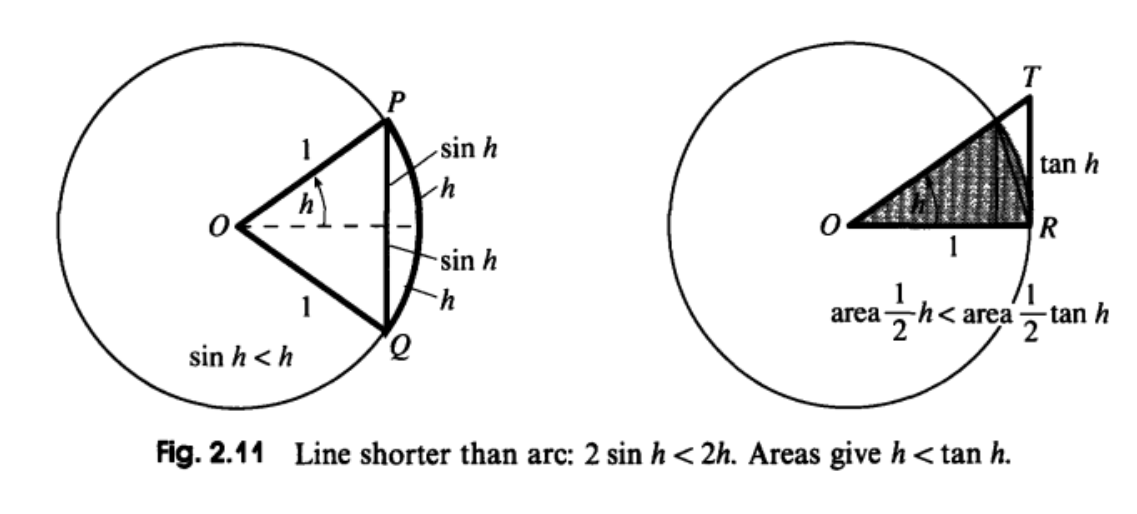
\includegraphics[width=0.9\textwidth]{33pic.png}
\end{center}
\item For $\lim_{h\rightarrow 0}\frac{\cos h-1}{h}$, use previous result by multiplying by the conjugate and show the limit is zero
\item Returning, both limits exits and we can use limit laws.
\begin{align*}
\frac{d}{dx}\sin(x) &= \cos x\lim_{h\rightarrow 0}\frac{\sin h}{h}+\sin x\lim_{h\rightarrow 0}\frac{\cos h-1}{h} 
= \cos(x) \cdot 1 + \sin(x) \cdot 0 = \cos(x)
\end{align*}
\item Note: $x$ must be in term of radians here, degrees differ in result by constant.
\item Important limits to take note of:
$$
\frac{\sin(\theta)}{\theta} = 1 \quad \text{and} \quad \lim_{h\rightarrow 0}\frac{\cos h-1}{h} = 0
$$
\end{enumerate}


%%%%%%%%%%%%%%%%%%%%%%%%%%%%%%%%%%%%%%%

%%%%%%%%%%%%%%%%%%%%%%%%%%%%%%%%%%%%%%%
\item Theorem: Derivative of all the trig functions ($\cos x$ is in homework 20, find others by yourself). Show these except cosine via quotient rule.
$$
\frac{d}{dx} \sin(x) = \cos(x), \quad
\frac{d}{dx} \cos(x) = -\sin(x), \quad
\frac{d}{dx} \tan(x) = \sec^2(x)
$$
$$
\frac{d}{dx} \csc(x) = -\csc(x)\cot(x), \quad
\frac{d}{dx} \sec(x) = \sec(x)\tan(x), \quad
\frac{d}{dx} \cot(x) = -\csc^2(x)
$$

%%%%%%%%%%%%%%%%%%%%%%%%%%%%%%%%%%%%%%%
\item {\bf Examples: }
\begin{enumerate}
\item $$\frac{d}{dx}\frac{\sec x\sin x}{e^x+\tan x}$$
\item Find the second derivative of $\sec x$\\
\item Find the 99th derivative of $\sin x$
\end{enumerate}

%%%%%%%%%%%%%%%%%%%%%%%%%%%%%%%%%%%%%%%
\item Above limit results can be useful in clever ways.
\begin{enumerate}
\item 
$$\lim_{\theta\rightarrow 0} \frac{\sin (7\theta)}{3\theta} = 
\lim_{\theta\rightarrow 0} \frac{\sin (7\theta)}{7\theta}\frac{7\theta}{3\theta} = \frac{7}{3}$$
\item Find 
$$\lim_{\theta\rightarrow 0} \frac{\sin(4x)}{\sin(6x)} = \frac{2}{3}$$
\item Mention limit law use and substitution ideas here.
\item Mention for future use.
$$\lim_{\theta\rightarrow \infty} \frac{\sin (\theta)}{\theta} = 0$$
\end{enumerate}
\end{enumerate}


%%%%%%%%%%%%%%%%%%%%%%%%%%%%%%%%%%%%%%%
%%%%%%%%%%%%%%%%%%%%%%%%%%%%%%%%%%%%%%%
\subsection{3.4 The chain rule}
How many differentiation rules do we have? List as many as they can say.
What are we missing? Combining functions via function composition.
$$
\frac{d}{dx}\sin(2x)=?
$$

\begin{enumerate}

%%%%%%%%%%%%%%%%%%%%%%%%%%%%%%%%%%%%%%%
%%%%%%%%%%%%%%%%%%%%%%%%%%%%%%%%%%%%%%%
\item Rate of change
\begin{enumerate}
\item A cheetah is 10x as fast as me. I am 2x as fast as my chicken. How much faster is the cheetah than my chicken? 20x as fast.
\item Example of temperature of La Crosse, temperature in the room, temperature in my storage case.
\item Explanation of chain idea: change in daytime light - changes - temperature - changes - growth of apple tree - changes - size of apple - changes - size of worm population
\item Draw classic function composition diagram, but write $y=f(g(x))$. Then, we have the chain rule. Rate of change in $f\circ g$ at $x$ is the same as ROC of $g$ at $x$ times ROC of $f$ at $g(x)$.
\end{enumerate}

%%%%%%%%%%%%%%%%%%%%%%%%%%%%%%%%%%%%%%%
\item Theorem: For $f$ and $g$ differentiable, $f\circ g$ is also differentiable and
$$
\frac{d}{dx} f(g(x)) = f'(g(x))g'(x)
$$
or equivalently in Leibniz notation.
$$
\frac{dy}{dx} = \frac{dy}{du} \frac{du}{dx}.
$$
\begin{enumerate}
\item Proof idea:
\[
\frac{d}{dx} f(g(x)) = \lim_{h \rightarrow 0} \frac{f(g(x+h)) - f(g(x))}{h} = \lim_{h \rightarrow 0} \frac{f(g(x+h)) - f(g(x))}{g(x+h)-g(x)}\frac{g(x+h)-g(x)}{h}
\]
then change of variable and done.
\item {\bf Example:} 
$$
f(x) = x^2,\quad g(x) = 2x
$$
\item More intuition:
\begin{enumerate}
\item {\bf Examples:} Carefully identify $f$ and $g$. Challenge is identifying inside and outside functions.  
$$(x^2+x+1)^{1000}, \quad \sin(1+\cos(x)), \quad \tan^3(4x)$$
\item This is a versatile new technique. Quotient rule revisited:
$$
\frac{d}{dx} \frac{f(x)}{g(x)} = \frac{d}{dx} f(x)(g(x))^{-1}
$$
\end{enumerate}
\item Differential equation: population, mass-spring
\end{enumerate}

%%%%%%%%%%%%%%%%%%%%%%%%%%%%%%%%%%%%%%%
\item General exponential functions 
\begin{enumerate}
\item $2^x = e^{\ln(2)x}$, now differentiate via the chain rule.
\item Theorem:
$$
\frac{d}{dx}a^x = a^x\ln (a)
$$
\item {\bf Example:} $$2^{3^{x^2}}$$
\item Do speed review of inverse functions and logarithmic function
\end{enumerate}
\end{enumerate}


%%%%%%%%%%%%%%%%%%%%%%%%%%%%%%%%%%%%%%%
%%%%%%%%%%%%%%%%%%%%%%%%%%%%%%%%%%%%%%%
\subsection{3.5 Implicit differentiation}
\begin{enumerate}

%%%%%%%%%%%%%%%%%%%%%%%%%%%%%%%%%%%%%%%
\item What remains?
\begin{enumerate}
\item Inverse trig function, $\ln(x)$ (next section via chain rule), curves which aren't functions.
\item Should be able to differentiate any curve via the same idea, just locally.
\end{enumerate}

%%%%%%%%%%%%%%%%%%%%%%%%%%%%%%%%%%%%%%%
\item Implicit differentiation (chain rule in disguise)
\begin{enumerate}
\item {\bf Examples:} Find $\frac{dy}{dx}$ for $x^2+y^2 =1$ (graph)
\begin{enumerate}
\item Idea: treat $y=y(x)$ and differentiate both sides of equation. Require chain rule for $y$ terms.
\item Is it useful? Just the same, but a bit more difficult to use. Find the equation of the tangent line of $x^2+y^2 = 1$ at $(\sqrt{2}/2,\sqrt{2},2)$
\item Note:
\begin{itemize}
\item Always have multiple of $y'$ for function $y$, actually the chain rule
\item Your answer may involve both $x$ and $y$
\item All the other rules apply just the same
\item Find the derivative by plugging in both $x$ and $y$. 
\end{itemize}
\end{enumerate}
\item {\bf Examples:} Find $\frac{dy}{dx}$ for $x^3+y^3 =6xy$ (Folium of Descartes)
\begin{enumerate}
\item Graph in desmos. Compare for following.
\item Show (3,3) is on the graph. What is $\frac{dy}{dx}|_{x=3}$?
\item Where is $\frac{dy}{dx}=0$? Undefined?
\end{enumerate}
\item {\bf Examples:} Find $\sin x\sin y+\sin y \sin x = 0$, draw the derivative in Desmos, nodal lines
\begin{itemize}
\item  Youtube: amazing resonance effect 
\item \url{https://www.youtube.com/watch?v=wvJAgrUBF4w&noredirect=1}
\item \url{https://www.youtube.com/watch?v=uENITui5_jU}
\end{itemize}
\item {\bf Examples:} Find $\frac{dy}{dx}$ for $\sin(x+y) = e^{xy}$
\item {\bf Examples:} Find the equation of the tangent line to $y\sin 2x = x\cos 2y$ at $(\pi/2, \pi/4)$
\item Can show the power rule for rational powers:
$$ y = x^n = x^{p/q}, \quad y^q = x^p, \quad qy^{q-1} \frac{dy}{dx} = px^{p-1}$$
\end{enumerate}

%%%%%%%%%%%%%%%%%%%%%%%%%%%%%%%%%%%%%%%
\item Derivatives of inverse trigonometric functions
\begin{enumerate}
\item {\bf Examples:} Find $y'$ for $\sin y = x$: $y' = \frac{1}{\sqrt{1-x^2}}$
\item Find all the inverse trig functions by yourself, we just did $\arcsin$. Short review below (not invertible, domain restriction, Pythagorean identities, etc)
\begin{itemize}
\item $\arcsin(x), \quad -\frac{\pi}{2} \leq x \leq \frac{\pi}{2}$
\item $\arccos(x), \quad 0 \leq x \leq \pi$
\item $\arctan(x), \quad -\frac{\pi}{2} < x < \frac{\pi}{2}$
\item $\text{arccsc}(x), \quad -\frac{\pi}{2} \leq x \leq \frac{\pi}{2}$
\item $\text{arcsec}(x), \quad 0 \leq x \leq \pi$
\item $\text{arccot}(x), \quad -\frac{\pi}{2} < x < \frac{\pi}{2}$
\end{itemize}
\item Add to your list of derivatives to know.
\item {\bf Examples:} Use two method to find the derivative ((students) chain rule, (me) draw triangle and simplify as algebraic expression).
$$
y = \sin(\cos^{-1} x)
$$
\end{enumerate}

%%%%%%%%%%%%%%%%%%%%%%%%%%%%%%%%%%%%%%%
\item Derivative of general inverse functions
\begin{enumerate}
\item Implicit differentiation, need not memorize this formula.
$$
y=f^{-1}(x), \quad f(y)=x, \quad (f^{-1}(x))' = \frac{1}{f'(f^{-1}(x))}
$$
\item Illustrate by graph, reflection across main diagonal, how does the slope of the tangent change, slope is the reciprocal?
\end{enumerate}
\end{enumerate}


%%%%%%%%%%%%%%%%%%%%%%%%%%%%%%%%%%%%%%%
%%%%%%%%%%%%%%%%%%%%%%%%%%%%%%%%%%%%%%%
\subsection{3.6 Derivative of logarithmic functions}
\begin{enumerate}

\item Historic motivational interestingness: \url{https://en.wikipedia.org/wiki/History_of_logarithms}

%%%%%%%%%%%%%%%%%%%%%%%%%%%%%%%%%%%%%%%
\item Theorem: (show via implicit differentiation of $x=e^y$)
$$
\frac{d}{dx}(\ln x) = \frac{1}{x}
$$
and
$$
\frac{d}{dx}(\log_a x) = \frac{1}{x\ln a}
$$
\begin{enumerate}
\item {\bf Examples:} (with the Chain rule)
\begin{enumerate}
\item $\frac{d}{dx} (\ln (-x))$
\item $\frac{d}{dx} (\log_5 (x^2 e^x))$ (2 ways, chain rule then log properties can be handy, need change of base formula to show match)
\item $\frac{d}{dx}(\ln |x|) = \frac{1}{x}$
\end{enumerate}
\end{enumerate}

%%%%%%%%%%%%%%%%%%%%%%%%%%%%%%%%%%%%%%%
\item Logarithmic differentiation: Logarithms are valued for their sweet properties.
\begin{enumerate}
\item Three nice property of $\log_a (x)$ (prod, quotient, powers), $\ln(x)$ is the nicest choice.
\item {\bf Example:} $y = x^x$, then $y'=?$ (no such rule)
\item {\bf Example:} $y = \frac{(x^2+1)(x+3)^{1/2}}{x-1}$, then $y'=?$ (quotient, product, chain rule madness)
\item Summary of steps: 
\begin{enumerate}
\item  Identify the situation (lots of multiplication, quotient, and powers)
\item Take log on both sides (if possible) and simplify using the log properties.
\item Differentiate implicitly with respect $x$
\item Solve for $y'$
\item What if $y=f(x)<0$ for some $x$? Use absolute value.
$$
|y|=|f(x)|, \quad \ln(|y|)=\ln(|f(x)|), \quad \frac{1}{y}\frac{dy}{dx} = \frac{1}{f(x)}f'(x), \quad \frac{dy}{dx}=\dots 
$$
\end{enumerate}
\item {\bf Example:} Finally, the full power rule: $y = x^n$, $n$ any real number, log differentiation.
\end{enumerate}

%%%%%%%%%%%%%%%%%%%%%%%%%%%%%%%%%%%%%%%
\item More complicated cases:
\begin{enumerate}
\item {\bf Examples:} Find $y'$ for 
$$
y = x^{x^x}, \quad y = \sin x^{\cos x}, \quad y = \Big(\frac{(2x+3)^2\sqrt{2-x}}{(x-1)^3}\Big)^{x^2}
$$
$$
y^x = x^y
$$
\end{enumerate}

%%%%%%%%%%%%%%%%%%%%%%%%%%%%%%%%%%%%%%%
\item Important results to know:
\begin{enumerate}
\item Theorem:
$$
\lim_{x\rightarrow 0} (1+x)^{1/x} = e
$$
Reason: $f(x)=\ln(x)$, then $f'(x)=\frac{1}{x}$ and $f'(1)=1$. So,
$$
1=f'(1)=\lim_{h\rightarrow 0} \frac{1}{h}\ln(1+h)=\lim_{h\rightarrow 0} \frac{\ln(1+h)}{h}=\lim_{h\rightarrow 0} \ln((1+h)^{1/h})
$$
Then, because exponential functions are continuous,
$$
\lim_{x\rightarrow 0}\ln(1+x)^{1/x} = 1 \quad \Rightarrow \quad e=e^1=e^{\lim_{x\rightarrow 0}\ln(1+x)^{1/x}} = \lim_{x\rightarrow 0} (e^{\ln(1+x)^{1/x}})=\lim_{x\rightarrow 0} (1+x)^{1/x}
$$
\item Corollary: Take $n=\frac{1}{x}$ above,
$$
e=\lim_{n\rightarrow \infty}(1+\frac{1}{n})^n \quad \text{(holy compound interest Batman!)}
$$
\item Continuous compounded interest: PERT all ova the place.
$$
\lim_{n\rightarrow \infty}P(1+\frac{r}{n})^{nt}  = Pe^{rt}
$$
\end{enumerate}
\end{enumerate}


%%%%%%%%%%%%%%%%%%%%%%%%%%%%%%%%%%%%%%%
%%%%%%%%%%%%%%%%%%%%%%%%%%%%%%%%%%%%%%%
\subsection{3.8 Exponential growth and decay}
\begin{enumerate}


%%%%%%%%%%%%%%%%%%%%%%%%%%%%%%%%%%%%%%%
\item Things that \emph{change} according to a rule (or rules) can be translated into a differential equation.  \\
 See the many examples:
\begin{itemize}
\item \url{https://en.wikipedia.org/wiki/Differential_equation}
\item \url{https://people.maths.ox.ac.uk/trefethen/pdectb.html}
\item Def: A differential equation is an equation involving derivatives where the unknown is a \emph{function}. (analogous to algebraic equations)
\end{itemize}


%%%%%%%%%%%%%%%%%%%%%%%%%%%%%%%%%%%%%%%
\item Exponential growth and decay is a simple start.
$$
\frac{dy}{dt} = ky, \quad y(0)=y_0
$$
Here $k$ is some constant ($k>0$ growth, $k<0$ decay) and $y_0$ is the initial size. $y=y(t)$ is an unknown function of time $t$ need to find.
\begin{enumerate}
\item Read the DE as 'quantity $y$ changes at a rate proportional to it's size'. What a language!
\item What things do you know which do this? Population, investment, radioactive decay, temperature of object, etc. Will see DEs in advanced related classes.
\item How to find solution $y(t)$? We already know a function whose derivative is (almost) the same. Guess $y(t)=Ce^{kt}$ for some constant $C$. Then,
$$
\frac{dy}{dt} = \frac{d}{dt}(Ce^{kt}) = ky 
$$
What is $C$?
$$
y(0) = C = y_0
$$
Then, the solution is $y(t)=y_0e^{kt}$. PERT formula!
\item Can show the ONLY solution to the above DE is $y(t)=y_0e^{kt}$ (uniqueness).
\end{enumerate}

%%%%%%%%%%%%%%%%%%%%%%%%%%%%%%%%%%%%%%%
\item {\bf Examples:} (Optional)
\begin{enumerate}
\item Population growth, La Crosse had population 50000 in 2000 and 55000 in 2010, what will the population be in 2020? Here we \emph{choose} the above model. What are the issues with this assumption? \\
Log plots: Google populations of california, texas, florida. \url{https://www.google.com/publicdata/explore?ds=kf7tgg1uo9ude_&met_y=population&idim=state:06000:48000&hl=en&dl=en#!ctype=l&strail=false&bcs=d&nselm=h&met_y=population&scale_y=lin&ind_y=false&rdim=country&idim=state:06000:48000:12000&ifdim=country&hl=en_US&dl=en&ind=false}
\item Newton's Law of Cooling: Newton said the rate at which an object cools (or warms) is proportional to the difference in temp of the object and its surrounding temp. Language sound familiar?
$$
\frac{dT}{dt} = k(T-T_s), \quad T(0)=T_0
$$
where $T(t)$ is the unknown temperature function. Ideal coke temp $38^{\circ}$
\item Solution: We've already solved this type once and for all! Use the substitution $y(t)=T(t)-T_s$ and reduce to $\frac{dy}{dt}=ky$.
\item Coffee example if in high demand.
\end{enumerate}
\end{enumerate}


%%%%%%%%%%%%%%%%%%%%%%%%%%%%%%%%%%%%%%%
%%%%%%%%%%%%%%%%%%%%%%%%%%%%%%%%%%%%%%%
\subsection{3.9 Related rates}
\begin{enumerate}

%%%%%%%%%%%%%%%%%%%%%%%%%%%%%%%%%%%%%%%
\item Motivation: A single phenomenon can give many different rates of change
\begin{enumerate}
\item A snowball is melting. What quantities are changing? Rates comparable? (Length vs area vs volume)
\url{https://www.youtube.com/watch?v=LNEBZ8ekU18}
\item A ladder is sliding down a wall, driving a car, GPS, so many here.
\item Suppose a snow ball is melting at a rate $40cm^3/sec$, how fast is the diameter shrinking when the radius is 4cm?
\begin{itemize}
\item How are these two quantities related? 
\item Know: $V=\frac{4}{3}\pi r^3$, $d=2r$
\item What is changing in time? $V=V(t), r=r(t), d=d(t)$
\item Differentiate equation (always implicit differentiation here)
\end{itemize}
\end{enumerate}

%%%%%%%%%%%%%%%%%%%%%%%%%%%%%%%%%%%%%%%
\item Steps to solve related rates problem. Straightforward, but needs care to detail else will wander.
\begin{enumerate}
\item Make sure it's not an optimization problem (-est, most, least)
\item Assign all the variables 
\item Express the rates in terms of derivative 
\item Find the rate given and the rate you want to solve
\item Find a equation associating all the quantities in (3)
\item Use implicit differentiation to take derivatives of the equation (related rates)
\item Substitute in the missing information and solve
\end{enumerate}

%%%%%%%%%%%%%%%%%%%%%%%%%%%%%%%%%%%%%%%

\item {\bf Example:} A ladder 10 ft long is sliding against a vertical wall. If the bottom of the ladder slides away from the wall at a rate of 1ft/s, how fast is the top of the ladder sliding down the wall when the bottom of the ladder is 6ft from the way?
\begin{enumerate}
\item Drawing picture is key, Pythagorean theorem is key.
\item What is the changing rate of $\theta$?
\end{enumerate}
\item {\bf Example:}  A street light is mounted at the top of a 15-ft-tall pole. A man 6 ft tall walks away from the pole with a speed of 5 ft/s along a straight path. How fast is the tip of his shadow moving when he is 40ft from the pole?

%%%%%%%%%%%%%%%%%%%%%%%%%%%%%%%%%%%%%%%
\item Groupwork from text problems, pg 248, problems
\begin{itemize}
\item 22 (pythagoras) Thus, the boat approaches the dock at $\frac{\sqrt{65}}{8} \approx 1.01$ meters/sec
\item 45 (trig right triangle) $\frac{10}{9}\pi$ km/min or 130 mph
\item 18 (similar right triangles)  decreasing at a rate of 0.6 meters/sec
\item 42 (two pyth theorem comb to get rope length) $-\frac{10}{\sqrt{133}} \approx -0.87$ ft/sec
\end{itemize}

%%%%%%%%%%%%%%%%%%%%%%%%%%%%%%%%%%%%%%%
\item Global positioning system story of related rates. Student at MIT. \url{http://www.pcworld.com/article/2000276/a-brief-history-of-gps.html}
\end{enumerate}

%%%%%%%%%%%%%%%%%%%%%%%%%%%%%%%%%%%%%%%
%%%%%%%%%%%%%%%%%%%%%%%%%%%%%%%%%%%%%%%
\subsection{3.10 Linear approximations and differentials }
\begin{enumerate}

%%%%%%%%%%%%%%%%%%%%%%%%%%%%%%%%%%%%%%%
\item Motivation and idea:
\begin{enumerate}
\item Practical questions: What is $\sqrt{4.1}$, $\sin(46^\circ)$?
\item Idea: Use the value of a function around a known $f(a)$ in a smart way.
\item Think of
$$
f'(a)=\lim_{x\rightarrow a}\frac{f(x)-f(a)}{x-a}
$$
When $x$ is close to $a$ they basically satisfies the relationship.
\end{enumerate}

%%%%%%%%%%%%%%%%%%%%%%%%%%%%%%%%%%%%%%%
\item Linear approximation: the linear (tangent line) approximation of $f$ at $a$ is 
$$
L(x) = f(a)+f'(a)(x-a)
$$
Also known as the linearization of $f$ at $a$. Compare to limit of difference quotient above.
\begin{enumerate}
\item Idea: $f(x)$ is ``locally" a line (around $a$), draw picture of $f$ and $L$
\item This is an approximation and may not be accurate at all
\begin{itemize}
\item depending on the original shape
\item depending on how close your $x$ is to $a$
\end{itemize}
\end{enumerate}

%%%%%%%%%%%%%%%%%%%%%%%%%%%%%%%%%%%%%%%
\item {\bf Examples:} Find the linearization of $\sqrt{x}$ at $4$
\begin{enumerate}
\item Use it to approximate $\sqrt{4.1}$, $\sqrt{4.5}$, $\sqrt{6}$ and compare to the real value.
\item Find $\sin(44^\circ)$, do the same thing.
\item In physics, $\sin x\approx x$ when $x$ is small. This is linearization.
\end{enumerate}

%%%%%%%%%%%%%%%%%%%%%%%%%%%%%%%%%%%%%%%
\item Differentials: 
$$
dy = f'(x) dx
$$
\begin{enumerate}
\item What is this? Reminds of $\frac{dy}{dx}=f'(x)$. What if treat as a ration?
\item Find the differential of $x^2$ at $x =2$. Pick different $dx$ and graph.
\item Difference between $dy$ and $\triangle y$. Actually, $dy=\delta L$.
\item This is close to the original conceptualization of calculus.
\end{enumerate}

%%%%%%%%%%%%%%%%%%%%%%%%%%%%%%%%%%%%%%%
\item {\bf Example:}  A sphere was measured and its radius was found to be 45 inches with a possible error of no more that 0.01 inches.  
What is the maximum possible error in the volume if we use this value of the radius?
\[
V = \frac{4}{3}\pi r^3 \quad \Rightarrow \quad \Delta V \approx dV = 4\pi r^2 dr
\]

%%%%%%%%%%%%%%%%%%%%%%%%%%%%%%%%%%%%%%%
\item Can we replace $f(x)$ locally by a quadratic equation?
\begin{enumerate}
\item Doable? (Yes, need first and second derivatives to match)
\item More work? (Yes)
\item Better accuracy? (Yes)
\item Any polynomial? (Taylor polynomial, calculus 2)
\item Why bother replacing functions with polynomials? (Biggest take-away of the section)
\begin{itemize}
\item Approximation of hard calculations
\item Polynomials are nicer functions than anything else, so live in a better place.
\end{itemize}
\item Can we use things other than polynomials? Sure thing (Fourier series) for periodic functions (light, sound, universe of waves).
\end{enumerate}
\end{enumerate}


%%%%%%%%%%%%%%%%%%%%%%%%%%%%%%%%%%%%%%%
%%%%%%%%%%%%%%%%%%%%%%%%%%%%%%%%%%%%%%%
\subsection{3.11 Hyperbolic functions}
\begin{enumerate}

%%%%%%%%%%%%%%%%%%%%%%%%%%%%%%%%%%%%%%%
\item Motivation:  
\begin{enumerate} 
\item Think about a heavy flexible cable suspended between two points at the same height (the golden gate bridge, telephone cable). This is called a catenary. What is that curve? Not quite a parabola.
\url{https://www.google.com/search?q=catenaries&espv=2&biw=1680&bih=921&tbm=isch&tbo=u&source=univ&sa=X&ved=0ahUKEwj5552K2ejKAhVCFR4KHRoADp8QsAQIQw#tbm=isch&q=catenary&imgrc=ES8GEHgRx3OpXM%3A}
$$
\frac{e^x+e^{-x}}{2}
$$
\item What's the derivative?
\end{enumerate}

%%%%%%%%%%%%%%%%%%%%%%%%%%%%%%%%%%%%%%%
\item The family of hyperbolic functions, such parallels with regular trigonomety here.
$$
\sinh x  = \frac{e^x-e^{-x}}{2},\quad\cosh x  = \frac{e^x+e^{-x}}{2}
$$
\begin{enumerate}
\item Regular division and such gives the rest. $\tanh(x)=, \dots$.
\item Just as the points $(\cos(t), \sin(t))$ form a circle with a unit radius, the points $(\cosh(t), \sinh(t))$ form the right half of the equilateral hyperbola $x^2-y^2=1$. 
\item For some applications, this is the correct geometry (special relativity).
\end{enumerate}

%%%%%%%%%%%%%%%%%%%%%%%%%%%%%%%%%%%%%%%
\item Hyperbolic identities:
\begin{enumerate}
\item Odd, even:
$$
\sinh(-x) = -\sinh(x),\quad \cosh(-x) = \cosh(x)
$$
\item The "Pythagorean" identities:
$$
\cosh^2 x-\sinh^2 x = 1,\quad 1-\tanh^2  = sech^2x
$$
\item The sum formula:
$$
\sinh(x+y) = \sinh(x)\cosh(y)+\cosh(x)\sin(y)
$$
$$
\cosh(x+y) = \cosh(x)\cosh(y)+\sinh(x)\sin(y)
$$
\item Double angle formula:
$$
\sinh(2x) = 2\sinh x\cosh x
$$
\end{enumerate}

%%%%%%%%%%%%%%%%%%%%%%%%%%%%%%%%%%%%%%%
\item Derivatives of hyperbolic functions (show this)
$$
(\sinh x)' = \cosh x
$$

%%%%%%%%%%%%%%%%%%%%%%%%%%%%%%%%%%%%%%%
\item Inversere hyperbolic function (show this, substitution, hidden quadratic)
$$
\sinh^{-1}(x) = \ln (x+\sqrt{x^2+1})
$$

\item What you need to know:
\begin{enumerate}
\item Know they come from application. Be aware.
\item You don't have to memorize anything but the definition of the hyperbolic sine and cosine.
\item Feel free to check the book when you do the homework
\item I may test it as an exercise of derivatives.
\end{enumerate}
\end{enumerate}


%%%%%%%%%%%%%%%%%%%%%%%%%%%%%%%%%%%%%%%
%%%%%%%%%%%%%%%%%%%%%%%%%%%%%%%%%%%%%%%
\section{Chapter 4 Applications of differentiation}

%%%%%%%%%%%%%%%%%%%%%%%%%%%%%%%%%%%%%%%
%%%%%%%%%%%%%%%%%%%%%%%%%%%%%%%%%%%%%%%
\subsection{4.1 Maximum and minimum values}

%%%%%%%%%%%%%%%%%%%%%%%%%%%%%%%%%%%%%%%
\begin{enumerate}
\item Motivation: Where do we see optimization
\begin{itemize}
\item
\item What's the maximum/minimum speed (speeding ticket? Why do you care?
\item Buying stocks, when to take action?
\item Suppose you have a fence of 100 ft long. How to fence a rectangular region so that the area is maximum?
\item What's biggest rectangle inside a circle?
\item Who is the best March madness basketball team?
\end{itemize}

%%%%%%%%%%%%%%%%%%%%%%%%%%%%%%%%%%%%%%%
\item Extreme values definition: Let $c$ be a number in the domain $D$ of a function $f$. Then
\begin{itemize}
\item $f(c)$ is the absolute maximum value of $f$ on $D$ if $f(c)\geq f(x)$ for all x in D
\item $f(c)$ is the absolute minimum value of $f$ on $D$ if $f(c)\geq f(x)$ for all x in D
\end{itemize}
\item Draw a graph typical to smooth nice functions already seen

%%%%%%%%%%%%%%%%%%%%%%%%%%%%%%%%%%%%%%%
\item True or False? (Keys: domain endpoints included/not, unbounded functions, discontinuities, singularities (corners), lots of cases here but not too many, draw pictures to summarize)
\begin{itemize}
\item Domain $D$ matters. 
\item $f$ can have more than 2 absolute values.
\item Every function must have an absolute value.
\item Absolute values occur where $f'(x)=0$.
\end{itemize}

%%%%%%%%%%%%%%%%%%%%%%%%%%%%%%%%%%%%%%%
\item Lots of possibilities: Which have absolute max or mins? What are they?
\begin{enumerate}
\item $f(x)=1/x$ (no domain listed implies all possible $x$.
\item $f(x)=x^2$
\item $f(x)=x^2$ on $[0,2]$
\item $f(x)=x^2$ on $(0,2)$
\item Keys: domain endpoints included/not, unbounded functions, discontinuities, singularities (corners), lots of cases here but not too many, draw pictures to summarize with endpoints, abs local min max/don't name, non differentiable, discontinuity.
\end{enumerate}

%%%%%%%%%%%%%%%%%%%%%%%%%%%%%%%%%%%%%%%
\item {\bf Extreme Value Theorem}: if $f$ is continuous on a closed interval $[a,b]$, then $f$ attains its extreme values on $[a,b]$
\begin{enumerate}
\item Check hypothesis before computing
\item If it fails, can you say no absolute values? Nope.
\item Require
\begin{itemize}
\item Continuous
\item Closed interval (all endpoints included)
\item The max, min can be at $a, b$
\item Absolute max/min can occur multiple times
\end{itemize}
\end{enumerate}

%%%%%%%%%%%%%%%%%%%%%%%%%%%%%%%%%%%%%%%
\item Local Extreme Values
\begin{enumerate}
\item {\bf Definition:} a number $f(c)$ is a 
\begin{itemize}
\item Local maximum value of $f$ if $f(c)\geq f(x)$ when $x$ is near $c$
\item Local minimum value of $f$ if $f(c)\leq f(x)$ when $x$ is near $c$
\end{itemize}
\item Distinctions:
\begin{itemize}
\item Difference between absolute extreme values and local extreme values (draw a picture to illustrate)
\item Is an absolute max also local max?
\item Why do we want these in applications? More important in some cases (stock market)
\end{itemize}
\end{enumerate}

%%%%%%%%%%%%%%%%%%%%%%%%%%%%%%%%%%%%%%%
\item How to identify locations of local / absolute extrema? Already classified the cases.
\begin{enumerate}
\item {\bf Definition:} A critical number of $f$ is a number $c$ in the domain of $f$ such that $f'(c) = 0$ or $f'(c)$ DNE. (all cases here, see them? Stationary points, singular points, end points)
\item Fermat's little theorem: if $f$ has a local max/min at $c$ and if $f'(c)$ exists, then $f'(c) = 0$. 
\item True or false?
\begin{itemize}
\item If f'(c) = 0, then f has a local maximum or minimum at c
\item If f has a local maximum or minimum at c, then f'(c) = 0
Both are false
\end{itemize}
\end{enumerate}

%%%%%%%%%%%%%%%%%%%%%%%%%%%%%%%%%%%%%%%
\item Finding critical numbers of 
\begin{enumerate}
\item $f(x)=2x-\tan x$ on $(-\pi,\pi)$
\item $g(x)= x^{1/3}-x^{-2/3}$
\end{enumerate}

%%%%%%%%%%%%%%%%%%%%%%%%%%%%%%%%%%%%%%%
\item Method: Find the absolute extreme values of $f$: the closed interval method.
\begin{enumerate}
\item Check the extreme values theorem hypothesis
\item Find all the candidates: Critical numbers
\begin{itemize}
\item Stationary points
\item Singular points
\item End points
\end{itemize}
\item Compare the $f$ values at all the candidates.
\item Take the largest/smallest ones (may be more than one) and write the answer in the format: $f(x)$ has an absolute value (~) at x = ( )
\end{enumerate}


%%%%%%%%%%%%%%%%%%%%%%%%%%%%%%%%%%%%%%%
\item {\bf Examples:} Find the absolute maximum and minimum values of each. Where is the absolute max/min and where does it occur?
\begin{enumerate}
\item $f(x) = x^3+x^2-x$ on $[-2,2]$. 
\item $f(x) = x^{\frac{2}{3}}$, no interval then add open / closed. Change to $x^\frac{1}{3}$
\item $f(x) = x + 2\cos(x)$ on $[-2\pi,\pi]$
\end{enumerate}
\end{enumerate}	



%%%%%%%%%%%%%%%%%%%%%%%%%%%%%%%%%%%%%%%
%%%%%%%%%%%%%%%%%%%%%%%%%%%%%%%%%%%%%%%
\subsection{4.2 The mean value theorem}
Write statements, then let them think about what it could mean.
\begin{enumerate}

%%%%%%%%%%%%%%%%%%%%%%%%%%%%%%%%%%%%%%%
\item {\bf Rolle's Theorem:} Let $f$ be a function that satisfies the following three hypotheses: 
\begin{itemize}
\item $f$ is continuous on the closed interval $[a,b]$
\item $f$ is differentiable on the open interval $(a,b)$
\item $f(a) = f(b)$
\end{itemize}
Then there's a number $c$ in $(a,b)$ such that $f'(c) = 0$. Once they sort out, draw picture. Why is this useful?
\begin{itemize}
\item Proof:
\item If $f$ is a constant function, we are done.
\item Assume $f(x)>f(a)$ for some $x$. Then by the etreme value theorem $f$ has a max value which must be a local max. Then $f'(c)=0$ by Fermat's theorem.
\item Case where $f(x)<f(a)$ is similar.
\end{itemize}

%%%%%%%%%%%%%%%%%%%%%%%%%%%%%%%%%%%%%%%
\item {\bf Example} Show that $x^3+x-1 = 0$ has only one real solution.
\begin{enumerate}
\item Using IVT on $[0,1]$ to show existence.
\item What if had 2 zeros on $(0,1)$, $f(a)=f(b)=0$? Then Rolle's theorem says there is $c$ in $(a,b)$ such that $f'(0)=0$. But, $f'(x)=3x^2+1$. So, can only have 1 zero.
\end{enumerate}

%%%%%%%%%%%%%%%%%%%%%%%%%%%%%%%%%%%%%%%
\item {\bf Mean Value Theorem:} Let f be a function that satisfies
\begin{itemize}
\item $f$ is continuous on [a,b]
\item $f$ is differentiable on (a,b)
\end{itemize}
then there's a number c in (a,b) such that 
$$
f'(c) = \frac{f(b)-f(a)}{b-a}
$$
\begin{enumerate}
\item Draw picture to illustrate, drr...
\item Pro0f: Reduce the situation to Rolle's Theorem. Let $g(x)$ be the line through $(a,f(a)), (b,f(b))$.
\[
g(x) = f(a) + \frac{f(b)-f(a)}{b-a} (x-a)
\]
Define $s(x)=f(x)-g(x)$. Rolle's theorem gives $s'(c)=0$ for some $c$ in $(a,b)$. Then, $f'(c)=\frac{f(b)-f(a)}{b-a}$.
\item Applications: 
\begin{itemize}
\item Average rate of change equals inst rat of change.
\item When you are driving, there'll always be a moment that your instantaneous velocity is the same as the average velocity.
\item Suppose you are driving from La Crosse to Madison: 150 mile, 1.5 hours. What should the speeding ticket be written for? 100mile/h
\end{itemize}
\end{enumerate}

%%%%%%%%%%%%%%%%%%%%%%%%%%%%%%%%%%%%%%%
\item {\bf Examples} Apply the Mean Value Theorem.
\begin{enumerate}
\item Show $(\cos A-\cos B) \leq (A-B)$.
\item If $f(0)=-3$ and $f'(x)\leq 5$ for all $x$, how large can $f(2)$ be?
\end{enumerate}

%%%%%%%%%%%%%%%%%%%%%%%%%%%%%%%%%%%%%%%
\item {\bf Theorem:} If $f'(x) =0$ for all $x$ in $(a,b)$, then $f$ is a constant on $(a,b)$. 
\begin{enumerate}
\item Why open interval here? Actual constant is not known. How to show this?
\item {\bf Proof:} Assume $f'(x)=0$ on $(a,b)$. Need to show for any $x_1,x_2$ in $(a,b)$, $f(x_1)=f(x_2)$. For $x_1<x_2$, by the MVT
\[
0 = f'(c) = \frac{f(x_1)-f(x_2)}{x_1-x_2}
\]
for some $c$ in $(x_1,x_2)$. Done.
\end{enumerate}


%%%%%%%%%%%%%%%%%%%%%%%%%%%%%%%%%%%%%%%
\item Antiderivative beginnings
\begin{enumerate}
\item Find $f(x)$ such that $f'(x) = 2x$. Lots here.
\item {\bf Corollary:} If $f'(x) = g'(x)$ for all $x$ in (a,b), then $f-g$ is a constant on (a,b)
\item That is: $f(x)$ is uniquely determined by $f'(x)$ subject to a change of constant. Terminology here is antiderivative.
\item {\bf Proof:} Let $h(x)=f(x)-g(x)$, then $h'(x)=0$. So $h(x)=C$ and $f(x)=g(x)+C$.
\end{enumerate}
\end{enumerate}


%%%%%%%%%%%%%%%%%%%%%%%%%%%%%%%%%%%%%%%
%%%%%%%%%%%%%%%%%%%%%%%%%%%%%%%%%%%%%%%
\subsection{4.3 How derivatives affect the shape of a graph}

%%%%%%%%%%%%%%%%%%%%%%%%%%%%%%%%%%%%%%%
\begin{enumerate}
\item {\bf Example:}
\begin{enumerate}
\item Graph $f(x)$, $f'(x)$ and $f''(x)$ for $f(x) = x^3+x^2-x$
\item How is $f'$ related to $f$, $f''$ to $f'$, $f''$ to $f$?
\end{enumerate}

%%%%%%%%%%%%%%%%%%%%%%%%%%%%%%%%%%%%%%%
\item First derivative $f'(x)$
\begin{enumerate}
\item {\bf Increasing/decreasing test}
\begin{itemize}
\item If $f'(x) >0$, then $f$ is increasing ($a<b$ gives $f(a)<f(b)$)
\item If $f'(x)<0$, then $f$ is decreasing ($a<b$ gives $f(a)>f(b)$)
\end{itemize}
\item {\bf The first derivative test} Suppose $c$ is a critical number for $f$ (possible local max/min). Let them fill in blank.
\begin{itemize}
\item If $f'(x)$ changes from positive to negative at $c$, then .... $f$ has a local max at $c$.
\item If $f'(x)$ changes from negative to positive at $c$, then .... $f$ has a local min at $c$.
\item If $f'(x)$ does not change sign at $c$, then .... $f$ has no local max or min at $c$.  (called a saddle point)
\end{itemize}
\end{enumerate}

%%%%%%%%%%%%%%%%%%%%%%%%%%%%%%%%%%%%%%%
\item  {\bf Examples: } Draw a number line and find the absolute and local maxs/mins for each. Plot the points.
\begin{enumerate}
\item $f(x) =3x^4-4x^3-12x^2+5$ 
\item $h(x) = 1+2\sin(x)$ on $[0,2\pi]$.
\item $g(x) = \sin(x)$ 
\item How to graph $f$? Have a pretty good picture. What else can we add for detail? Where are turning points? Zeros?
\end{enumerate}

%%%%%%%%%%%%%%%%%%%%%%%%%%%%%%%%%%%%%%%
\item Second derivative $f''(x)$, take $\sin x$ as an example. Let them fill in blank.
\begin{enumerate}
\item {\bf Concavity test}
\begin{itemize}
\item If ... $f''(x)>0$, then $f$ is  concave up
\item If ... $f''(x)<0$, then $f$ is  concave down
\end{itemize}
\item Application: Filling a coke bottle with a constant volume of pouring. How does the height function change in concavity?
\item {\bf The second derivative test: }
\begin{itemize}
\item $f'(c) = 0$, $f''(c) >0$, local min
\item $f'(c)=0$, $f''(c)<0$, local max
\end{itemize}
\item Used to find local max/min, easier than first derivative test.
\item If $f''(x)=0$, it's inconclusive. Why? Think of a graph. This is an inflection point.
\item When can't the second derivative test be used? If $f''$ does not exist (corner)
\end{enumerate}

%%%%%%%%%%%%%%%%%%%%%%%%%%%%%%%%%%%%%%%
\item {\bf Examples:} Graph sketching
\begin{enumerate}
\item Give a random graph and decide where it's increasing, decreasing, concave up/down, local max/min, inflection points.
\item Give a random graph of $f'$ and decide increasing, decreasing, concave up/down, local max/min, inflection points.
\item Sketch the graph of $3x^4-4x^3-12x^2+5$ with all detail and glory.
\item  Sketch the graph of 
$$
f(x) = x^{2/3}(6-x)^{1/3}\quad \text{ knowing } \quad f'(x) = \frac{4-x}{x^{1/3}(6-x)^{2/3}},\quad f''(x) = \frac{-8}{x^{4/3}(6-x)^{5/3}}
$$
\end{enumerate}
\end{enumerate}



%%%%%%%%%%%%%%%%%%%%%%%%%%%%%%%%%%%%%%%
%%%%%%%%%%%%%%%%%%%%%%%%%%%%%%%%%%%%%%%
\subsection{4.4 Indeterminate forms and L'Hospital Rule}

\begin{enumerate}
%%%%%%%%%%%%%%%%%%%%%%%%%%%%%%%%%%%%%%%
\item We've already seen indeterminate forms for limits, but here we get a better way to handle them.
\begin{enumerate}
\item {\bf Examples:} ...from the past...
\begin{itemize}
\item $\ds \lim_{x\rightarrow 1} \frac{x^2-1}{x-1}=1 \quad$ (0/0 IF, factor and cancel, hole in graph. )
\item $\ds \lim_{x\rightarrow 1} \frac{\ln(x)}{x-1}=? \quad$ (0/0 IF, cannot factor)
\end{itemize}
\item Key: Indeterminate forms can be ANYTHING. Modify above example to show 2, 200, $\pi$, $\infty$, 0, etc.
\item Types of indeterminate form:
\begin{itemize}
\item Type $0/0$
\item Type $\infty/\infty$
\item Type $0\cdot \infty$
\item Type $\infty-\infty$
\item Type $0^0, 1^\infty$, $\infty^0$
\end{itemize}
\end{enumerate}

%%%%%%%%%%%%%%%%%%%%%%%%%%%%%%%%%%%%%%%
\item {\bf Theorem: l'Hospital's Rule} If
\begin{enumerate}
\item $f$ and $g$ are differentiable in interval $I$ containing $x=a$, and
\item $\displaystyle\lim_{x\rightarrow a} \frac{f(x)}{g(x)}$ is of indeterminate form $0/0$ or $\infty/\infty$
\end{enumerate}
then
$$
\lim_{x\rightarrow a} \frac{f(x)}{g(x)} = \lim_{x\rightarrow a} \frac{f'(x)}{g'(x)}
$$
if $\displaystyle\lim_{x\rightarrow a} \frac{f'(x)}{g'(x)}$ exists or is $\pm\infty$

\begin{enumerate}
\item Why is this nice? $\ds \lim_{x\rightarrow 1} \frac{x^2-1}{x-1}=1, \lim_{x\rightarrow 1} \frac{\ln(x)}{x-1}=? \quad$ (0/0 IF, can use l'Hospital's Rule)
\item Why is LR true? {\bf Proof} idea for 0/0 case by graph (slope over slope).
\[
\frac{f(x)}{g(x)} \approx \frac{L_f(x)}{L_g(x)} = \frac{m_f(x-a)}{m_g(x-a)} = \frac{m_f}{m_g} = \frac{f'(a)}{g'(a)} \quad \text{since } f(a)=g(a)=0
\]
\item {\bf Proof} of $\infty/\infty$ case: $\frac{f(x)}{g(x)} = \frac{1/g(x)}{1/f(x)}$ transfers to 0/0 IF.
\item Note: LR works for one sided limits also
\end{enumerate}

%%%%%%%%%%%%%%%%%%%%%%%%%%%%%%%%%%%%%%%
\item {\bf Examples:}
\begin{enumerate}
\item Can get crazy: Which grows faster, $x^{1000}$ or $e^x$? How to tell? Look at the ratio: $\ds \lim_{x\rightarrow \infty} \frac{x^{1000}}{e^x}$
\item Old limits are easier (?):
$$
\lim_{x\rightarrow 0} \frac{\sqrt{1+x}-1}{x} = \frac{1}{2}, \quad \lim_{x\rightarrow 0 } \frac{\sin x}{x} = 1,\quad 
\lim_{x\rightarrow 0} \frac{\sin 2x}{\sin 3x} = 2/3
$$
\item Beware of temptation: 
\begin{enumerate}
\item $\lim_{x\rightarrow 0 }\cos x/x = 0$ What went wrong? What should I have had? ALWAYS check the hypothesis of LR first.
\item $\lim_{x\rightarrow \infty} \frac{\sqrt{x^2-1}}{x} = ?$, $\lim_{x \rightarrow \infty} \frac{\sqrt{9x+1}}{\sqrt{x+1}}$
\item $\lim_{x\rightarrow \infty} \frac{x+\sin(x)}{x} = 1$ cannot apply right away.
\end{enumerate}
\end{enumerate}

%%%%%%%%%%%%%%%%%%%%%%%%%%%%%%%%%%%%%%%
\item Other indeterminate forms: Idea is to always transfer to $0/0$ or $\infty/\infty$ form.
\begin{enumerate}
\item $0\cdot\infty$ IF, for the second one way works but not other.
$$
\lim_{x\rightarrow 0^+}x\ln(x), \lim_{x\rightarrow -\infty}xe^x
$$
\item $\infty - \infty$ IF
$$
\lim_{x\rightarrow 0} \cot x -1/x
$$
\item $0^0, \infty^0, 1^\infty$ IFs, cannot use algebra but logarithms are useful.
$$
\lim_{x\rightarrow 0 }x^x, \lim_{x\rightarrow \infty }(1+\frac{1}{x})^x
$$
Idea: $\ds \lim_{x\rightarrow \infty} [f(x)]^{g(x)} =\lim_{x\rightarrow \infty} e^{\ln([f(x)]^{g(x)})} = e^{\lim_{x\rightarrow \infty} g(x)\ln(f(x))}$ assuming limit exists since $e^x$ is continuous.

%%%%%%%%%%%%%%%%%%%%%%%%%%%%%%%%%%%%%%%
\item {\bf Examples:} 
$$
\lim_{x\rightarrow 0^+ } \frac{e^x-1}{\cos x} = 0
$$
$$
\lim_{x\rightarrow 1} \frac{\sin (x-1)}{x^2+x-2} = 1/3
$$
$$
\lim_{x\rightarrow \pi/2 } \frac{1-\sin x}{1+\cos 2x} = 1/4
$$
$$
\lim_{t\rightarrow 0^+ } (1+\sin 4t)^{\cot t}= e^4
$$
\item Mention it's super important: indeterminant form is the most common case we want to work on. (derivative, def integral, etc)
\end{enumerate}
\end{enumerate}



%%%%%%%%%%%%%%%%%%%%%%%%%%%%%%%%%%%%%%%
%%%%%%%%%%%%%%%%%%%%%%%%%%%%%%%%%%%%%%%
\subsection{4.5 Summary of carve sketching}
\begin{enumerate}

%%%%%%%%%%%%%%%%%%%%%%%%%%%%%%%%%%%%%%%
\item Guidelines for curve sketching (we've already covered this!):
\begin{enumerate}
\item Find the omain
\item Locate $x$ and $y$ intercepts
\item Does $f$ have symmetry (even or odd)?
\item Asymptotes (horizontal, vertical, oblique)
\item Where is $f$ increasing / decreasing?
\item Find local mins and maxes (critical pts and 1st or 2nd derivative test)
\item Concavity and points of inflection 
\item Put all together to get a fantastic picture
\end{enumerate}

%%%%%%%%%%%%%%%%%%%%%%%%%%%%%%%%%%%%%%%
\item {\bf Examples:}
\begin{enumerate}
\item $f(x) = \frac{1+2x^2}{1-x^2}$ (horizontal and vertical asymptotes)
\item $ g(x) = \frac{-3x^2+2}{x-1}$ (oblique asymptote, need long division)
\end{enumerate}
Read the section and finish the homework!
\end{enumerate}


%%%%%%%%%%%%%%%%%%%%%%%%%%%%%%%%%%%%%%%
%%%%%%%%%%%%%%%%%%%%%%%%%%%%%%%%%%%%%%%
\subsection{4.7 Optimization problmes}
This section is all about maximizing / minimizing some quantity subject to a given constraint. These problems are everywhere, some are just disguised (instructor scheduling problem, linear prog, genetic algorithm) 

\begin{enumerate}
%%%%%%%%%%%%%%%%%%%%%%%%%%%%%%%%%%%%%%%
\item A farmer has 800 ft of fence and wants to fence off a rectangular field. How to arrange the fence so that it covers the biggest area? What if one side was my 60ft house? Almost the same.

%%%%%%%%%%%%%%%%%%%%%%%%%%%%%%%%%%%%%%%
\item Optimization problem strategy:
\begin{enumerate}
\item Make sure it's an optimization problem (-est, most, least)
\item Draw a picture to help
\item Find the variable $y$ that you want to minimize/maximize, introduce other notation
\item Find the changing variable $x$
\item Write $y = f(x)$ as a function of $x$, eliminate other variables if needed
\item Identify an closed interval for $x$ (why necessary? Extreme Value Theorem)
\item Find the extreme value of $y$
\item Answer the original question in words
\end{enumerate}

%%%%%%%%%%%%%%%%%%%%%%%%%%%%%%%%%%%%%%%
\item {\bf Examples:}
\begin{enumerate}
\item A cylindrical can is required to hold $1$ liter of oil. Design the can to minimize the use of material. 
\[
S = 2\pi r^2 + 2\pi r h, \text{ (eliminate $h$, can also use implicit diff)}
\]
\item Find the point on the curve $ y = 2x-1$ closest to the point (3, 2). 
\[
d = \sqrt{(x-2)^2+(y-2)^2}, \text{ (can eliminate or implicit diff)}
\]
\item What's the area of the biggest rectangle that can be inscribed inside a unit circle?
\[
A = 2xy = 2x\sqrt{1-x^2}
\]
\end{enumerate}
\item So many applications here, especially in business.
\end{enumerate}


%%%%%%%%%%%%%%%%%%%%%%%%%%%%%%%%%%%%%%%
%%%%%%%%%%%%%%%%%%%%%%%%%%%%%%%%%%%%%%%
\subsection{4.8 Newton's method}

\begin{enumerate}
%%%%%%%%%%%%%%%%%%%%%%%%%%%%%%%%%%%%%%%
\item {\bf Motivating Example} Solve $x^3-3x+1 = 0$
\begin{itemize}
\item Pick place to start: $x_0 = 0$
\item Find the linearization at $(x_0, y_0)$
\item Follow linearization to get zero which approximates $f$'s zero.
\item Show Desmos right away
\item Write down the formula
$$
x_{n+1} = x_n -\frac{f(x_n)}{f'(x_n)}
$$
\item Do the iteration by hand
\item Do $x_0 = 7$, $4$.
\end{itemize}

%%%%%%%%%%%%%%%%%%%%%%%%%%%%%%%%%%%%%%%
\item Idea of Newton's method
\begin{enumerate}
\item Again, replace $f$ by linearization (calculus), sweet move.
\item Does it always work? What could go wrong? We need more than just a formula.
\begin{enumerate}
\item Could be no root at all (IVT to check existence)
\item Could hit zero derivative, shoot to infinity (zero division)
\item Find wrong root. 
\item Even though the formula stays the same, the result depends on the initial value $x_1$
\item Slows down at roots with multiplicity.
\item Sometimes it just doesn't work (MVT, diverges to infinity)
$$
x^{1/3}=0, \quad x_1 = 1.
$$
\item Under the right assumptions (continuous and differentiable around the root, choose $x_1$ close enough), can prove Newton's method is fast and effective.
\end{enumerate}
\end{enumerate}

%%%%%%%%%%%%%%%%%%%%%%%%%%%%%%%%%%%%%%%
\item Find the solution of $\cos x = x$ using the Newton's method
\begin{enumerate}
\item Draw a picture to see how many solutions are there
\item Find the iteration method
\item For which initial value does it fail
\item Assign the initial value 
\item Compute the result
\item Mention fixed point methods if interested $x_n = \cos(x_{n-1})$
\end{enumerate}

%%%%%%%%%%%%%%%%%%%%%%%%%%%%%%%%%%%%%%%
\item Mind-blowing awesomeness:
\begin{enumerate}
\item \url{http://octave-online.net/}
\item $\sqrt{2}$ via $x^2=2$.
\item $\pi$ via $\sin(x)=0$ fast, $\cos(x)=1$ slow. Why? Multiplicity of root.
\item R pseudocode:
\begin{verbatim}
# newton's method
options(digits=16)

f <- function(x){x^2-2}
fp <- function(x){2*x}

x <- 1
for (i in c(1:10)){
  x <- x - f(x)/fp(x)
  print(x)
}
\end{verbatim}
\end{enumerate}

%%%%%%%%%%%%%%%%%%%%%%%%%%%%%%%%%%%%%%%\item More
\begin{enumerate}
\item How to improve on Newton? Taylor series to higher order
\item Fractals and complex numbers
\begin{itemize}
\item Zoomin: \url{https://www.youtube.com/watch?v=0jGaio87u3A}
\item Applications: \url{https://en.wikipedia.org/wiki/Fractal#Applications_in_technology}
\item Nature: \url{https://www.google.com/search?q=fractal+nature&espv=2&biw=1309&bih=781&tbm=isch&tbo=u&source=univ&sa=X&ved=0ahUKEwjS677XsIbMAhUMMSYKHSwkBC0QsAQIGw}
\end{itemize}
\end{enumerate}
\end{enumerate}


%%%%%%%%%%%%%%%%%%%%%%%%%%%%%%%%%%%%%%%
%%%%%%%%%%%%%%%%%%%%%%%%%%%%%%%%%%%%%%%
\subsection{4.9 Anti-derivatives}
\begin{enumerate}

%%%%%%%%%%%%%%%%%%%%%%%%%%%%%%%%%%%%%%%
\item Motivation: Goal is to reverse differentiation. Key here is lack of uniqueness.
\begin{enumerate}
\item Zombies touched on this situation already, leads to predator prey.
\item Find function $F(x)$ such that $F'(x) = 2x$
\item What about $F'(r) = 2\pi r$?, $F'(r) = 4\pi r^3$? Wha??
\item Conservation law.
\item Free fall $a(t) = 9.8 m/s^2$, can get velocity and distance.
\item Free fall with drag $a(t) = 9.8 - kv$ (gravity const - drag).
\item Kepler's laws of planetary motion spurred Newton to work on Calculus and support theory of physics.
\item Any physical (or other) law.
\end{enumerate}

%%%%%%%%%%%%%%%%%%%%%%%%%%%%%%%%%%%%%%%
\item {\bf Def:} Function $F$ is an antiderivative of $f$ on interval $I$ if $F'(x) = f(x)$ for all $x$ on $I$.
Comments
\begin{enumerate}
\item Note: An antiderivative is not unique. Why?
\begin{itemize}
\item Graphically, the derivative only tells you the shape of the function subject to a vertical shift
\item By computation, differentiating a constant always gives zero.
\item Mean value theorem already gave us this as a theorem (lemma?).  If $F$ is an anti-derivative of $f$ on an interval $I$, then the most general anti-derivative of $f$ on $I$ is $$
F(x)+C
$$
were C is an arbitrary constant.
\end{itemize}
\end{enumerate}

%%%%%%%%%%%%%%%%%%%%%%%%%%%%%%%%%%%%%%%
\item How to understand $F(x)+C$? 
\begin{enumerate}
\item Give me three examples for function $F$ you choose. 
\item How to make it unique? Need more information. Find the anti-derivative of  $f(x)=2x$ that passes through point $(0,1)$. Also, zombies already tackled this situation.
\end{enumerate}

%%%%%%%%%%%%%%%%%%%%%%%%%%%%%%%%%%%%%%%
\item A new idea handles this lack of uniqueness. \\
{\bf Definition:} The set of all antiderivatives of a function is called the indefinite integral of $f$ with respect to $x$, written
$$
\int f(x) ~dx = F(x) + C
$$
where $C$ is an arbitrary constant. The process of computing integrals is integration. Here, we see differential notation and a stretched out S, reasons to come.

%%%%%%%%%%%%%%%%%%%%%%%%%%%%%%%%%%%%%%%
\item Properties of the indefinite integral come from differentiation. They are easily checked through that lens.
\begin{enumerate}
\item $\ds \int cf(x) ~dx = c\int f(x) ~dx$
\item $\ds \int f(x) + g(x) ~dx = \int f(x) ~dx + \int g(x)~ dx$
\end{enumerate}

%%%%%%%%%%%%%%%%%%%%%%%%%%%%%%%%%%%%%%%
\item {bf Examples:} Find the anti-derivatives of each. List all differentiation rules. Note each are easily checked, though integration is generally much harder than integration!
\begin{enumerate}
\item Integration rules: $k, x^n, \frac{1}{x}, \sin(x), \cos(x), \sec^2(x), \csc^2(x), \sec(x)\tan(x), \csc(x)\cot(x), e^x, e^{kx}, a^x, \frac{1}{1+x^2}$
\item $3x$
\item $x^2+e^x$
\item $xe^x$
\item $2x\cos(x^2)$
\item $\frac{2x}{1+x^2}$
\item Find $F(x)$ such that $F''(x) = x^2$
\item Find $f$ such that $f'(x) = \frac{x^2-x+5x^3}{2x}$ and $f(1)=2$.
\end{enumerate}
\end{enumerate}


%%%%%%%%%%%%%%%%%%%%%%%%%%%%%%%%%%%%%%%
%%%%%%%%%%%%%%%%%%%%%%%%%%%%%%%%%%%%%%%
\section{Chapter 5}

%%%%%%%%%%%%%%%%%%%%%%%%%%%%%%%%%%%%%%%
\subsection{5.1 Areas and distances}
Motivation:
\begin{itemize}
\item The area of a parabola
\item The area of a cylinder
\item The volume of a half sphere and a cylinder with a cone removed.
\item The area of two triangles between two parallel line
\item The contradiction between two triangles.
\end{itemize}
\begin{enumerate}

%%%%%%%%%%%%%%%%%%%%%%%%%%%%%%%%%%%%%%%
\item Recall, when we motivated this class, we had 2 main questions:
\begin{enumerate}
\item Tangent problem (derivative)
\item Area problem (our change of focus, definite integral)
\item Surprisingly, these are deeply connected.
\item Example: Driving car at 60mph. Draw displacement and velocity. What is the connection back and forth?
\begin{itemize}
\item $v'(t) = s(t)$
\item Accumulated area under $s$ gives function values of $v$.
\end{itemize}
\end{enumerate}

%%%%%%%%%%%%%%%%%%%%%%%%%%%%%%%%%%%%%%%
\item Find areas: Generally not so easy....
\begin{enumerate}
\item Rectangle, triangle, circle (talk Archimedes and limiting process)
\item Find the area under the curve $y = x^2+1$ on $[0,2]$. Use a simple shape (rectangle) to approximate. Draw idea by hand.
\item Use Desmos to show Riemann sum, emphasize limiting procedure, hint at indeterminate form. \url{https://www.desmos.com/calculator/tgyr42ezjq}
\end{enumerate}

%%%%%%%%%%%%%%%%%%%%%%%%%%%%%%%%%%%%%%%
\item Riemann Sum: Limiting procedure for area calculations. 
\begin{itemize}
\item Interval: $[a,b]=[0,2]$
\item Function $f(x)=x^2+1>0$ on $[a,b]$
\item Find the area under curve $y=f(x)$ (between $f(x)$ and the $x$-axis) on $[a,b]$
\end{itemize}
`
%%%%%%%%%%%%%%%%%%%%%%%%%%%%%%%%%%%%%%%
\begin{enumerate}
\item Finding the approximate area:
\begin{enumerate}
\item Partition of [a,b]
\item Find the area of each rectangle
\item Take the sum
\end{enumerate}

%%%%%%%%%%%%%%%%%%%%%%%%%%%%%%%%%%%%%%%
\item Details:
\begin{enumerate}
\item Divide $(a,b)$ into $n$ sub-intervals
\item Name all the ending points $x_0$, $x_1$,  ... , $x_n$
\item On each part, find the area of the rectangle
\begin{itemize}
\item Width: $\Delta x = (b-a)/n$, uniform for simplicity.
\item Height: for the $i_{th}$ rectangle, we have choices. 3 standard ways.
\begin{itemize}
\item Left ending points: $h_i = f(x_{i-1})$
\item Right ending points: $h_i = f(x_i)$
\item Midpoints: $h_i = f\left(\frac{1}{2}(x_{i-1})+f(x_{i})\right)$
\end{itemize}
\item Area of each rectangle: $A_i=h_i\cdot \Delta x$
\end{itemize}
\item Take the sum: 
$$
R_n = [h_1\cdot \Delta x+h_2\cdot \Delta x...+h_n\cdot \Delta x]
$$
\end{enumerate}
\item For the true area, take $n\rightarrow \infty$
$$
A = \lim_{n\rightarrow \infty} R_n
$$ 
\end{enumerate}

%%%%%%%%%%%%%%%%%%%%%%%%%%%%%%%%%%%%%%%
\item Formal (make it look better)
\begin{enumerate}

%%%%%%%%%%%%%%%%%%%%%%%%%%%%%%%%%%%%%%%
\item Height $h_i = f(x_i^*)$
\begin{itemize}
\item Left ending points: $x_i^* = x_{i-1}$
\item Right ending points: $x_i^* = x_i$
\item Midpoint: $x_i^* = (x_{i-1}+x_i)/2$
\item Does the answer depends on which sample we pick?
\begin{itemize}
\item For approximation (finite number of rectangles), yes it does.
\item Doesn't matter much when $n\rightarrow \infty$ as long as $f(x)$ is continuous.
\end{itemize}
\end{itemize}

%%%%%%%%%%%%%%%%%%%%%%%%%%%%%%%%%%%%%%%
\item Compactify the summation formula of $R_n$: Sigma notation.
\begin{itemize}
\item Review
$$
\sum_{i=1}^5 i^2,\quad 3, \quad j, \quad \sum_{c =1}^4 calculus
$$
\item Summation formulas: 
$$
\sum_{i=1}^n c = cn, \quad \sum_{i=1}^n i = \frac{n(n+1)}{2} (\text{Gauss, telescoping via} (i+1)^2-i^2 = 2i+1)
$$
$$
\quad \sum_{i=1}^n i^2 = \frac{n(n+1)(2n+1)}{6}, \quad \sum_{i=1}^n i^3 = \left(\frac{n(n+1)}{2} \right)^2
$$

%%%%%%%%%%%%%%%%%%%%%%%%%%%%%%%%%%%%%%%
\item Riemann sum
$$
R_n = \sum_{i=1}^n f(x_i^*)\Delta x
$$
\item Point to different notations and ask people the meaning of each term
\item Area = the limit of the Riemann sum: 
$$
A = \lim_{n\rightarrow\infty} R_n = \lim_{n\rightarrow\infty} \sum_{i=1}^n f(x_i^*)\Delta x
$$
\end{itemize} 
\end{enumerate}

%%%%%%%%%%%%%%%%%%%%%%%%%%%%%%%%%%%%%%%
\item {Examples:}
\begin{enumerate}
\item Find the approximate area under the graph of $f(x)=x^2+1$ on $[0,2]$ using 4 left/right rectangles. 
\item Find the approximate area under the graph of $\cos x$ from $(-\pi/2,\pi/2)$ using 
\begin{itemize}
\item 6 left rectangles
\item 6 right rectangles
\end{itemize}
\item Find the approximate area under the graph of $f(x)=x^2+1$ on $[0,2]$ using $n$ right rectangles. Take the limit to get true.
\end{enumerate}
\end{enumerate}


%%%%%%%%%%%%%%%%%%%%%%%%%%%%%%%%%%%%%%%
%%%%%%%%%%%%%%%%%%%%%%%%%%%%%%%%%%%%%%%
\subsection{5.2 The definite integral}
\begin{enumerate}

%%%%%%%%%%%%%%%%%%%%%%%%%%%%%%%%%%%%%%%
\item Goal: Find the exact area of $f(x)$ on $[a,b]$. \\
Idea: Take the limit of $R_n$ as $n\rightarrow \infty$.

%%%%%%%%%%%%%%%%%%%%%%%%%%%%%%%%%%%%%%%
\item  Definite integral of  $f$ from $a$ to $b$
$$
\int_a^b f(x)~dx = \lim_{n\rightarrow \infty} \sum_{i=1}^n f(x_i^*)\Delta x
$$
Provided  the limit exists.
\begin{itemize}
\item It's a limit of a sum
\item It's a number
\item Notation is complex. Keep reading it for what it is. Here it is clear why we use $\int$ to denote sum and $dx$ in place of $\Delta x$. Analogy here with differentials.
\item Terminology:
\begin{itemize}
\item Integrand: f(x)
\item Upper limit: b
\item Lower limit: a
\item Integration
\end{itemize}
\item Net area has physical meaning
\begin{itemize}
\item Positive
\item Negative
\item Cancellation (sine curve)
\item Give random functions and determine whether its net area is positive or negative
\end{itemize}
\end{itemize}

%%%%%%%%%%%%%%%%%%%%%%%%%%%%%%%%%%%%%%%
\item {\bf Examples:} We already computed one definite integral in previous section. Try this one on own via $x_i^*$ (1) left end points, (2) right end points. Check your work via geometry. One triangle subtract another.
$$
\int_{-1}^3 (-2x+4)~dx
$$
What if we had $\int_{-1}^5 (-2x+4)~dx$? Can use symmetry to get zero.

%%%%%%%%%%%%%%%%%%%%%%%%%%%%%%%%%%%%%%%
\item {\bf Examples:} Write the following expressions in terms of limit of a sum
$$
\int_0^1 \sin x~dx, \quad \int_{-2}^2 e^x\tan x~dx
$$

%%%%%%%%%%%%%%%%%%%%%%%%%%%%%%%%%%%%%%%
\item {\bf Examples:} Write the limit as definite integrals
\begin{itemize}
\item
$$
\lim_{n\rightarrow \infty}\sum_{i=1}^n x^*_i\sin x^*_i\frac{2}{n},\quad \text{with lower limit 0}
$$
\item
$$
\lim_{n\rightarrow \infty}\sum_{i=1}^n 3x^*_i\sqrt{x^*_i+1}
\frac{7}{n},\quad \text{with upper limit 4}
$$
\item
$$
 \lim_{n\rightarrow \infty}\sum_{i=1}^n \frac{\sin (x_i^*)^2}{\ln (x_i^*-2)}\Delta x,\quad \text{on}\quad [1,5]
$$
\end{itemize}

%%%%%%%%%%%%%%%%%%%%%%%%%%%%%%%%%%%%%%%
\item Properties of the definite integral
\begin{enumerate}
\item 
$$
\int_a^a f(x)dx = 0 \quad \text{no area}
$$
\item  $$
\int_a^b f(x)dx = \int_a^c f(x)dx+\int_c^b f(x)dx \quad \text{separate the interval}
$$
\item 
$$
\int_a^b f(x)dx = -\int_b^a f(x)dx  \quad \text{reverse direction}
$$
\item 
$$
\int_a^b c ~dx  = c(b-a),\quad\text{rectangular area is easy}
$$
\item 
$$
\int_a^b [f(x)+g(x)]dx = \int_a^b f(x)dx+\int_a^b g(x)dx  \quad \text{same as with summation}
$$
\item 
$$
\int_a^b [f(x)-g(x)]dx = \int_a^b f(x)dx-\int_a^b g(x)dx \quad \text{same as with summation}
$$
\item 
$$
\int_a^b [cf(x)]dx = c\int_a^b f(x)dx,\quad\text{where c is a constant}
$$
\end{enumerate}

%%%%%%%%%%%%%%%%%%%%%%%%%%%%%%%%%%%%%%%
\item Comparison properties of the integral (draw pictures with each)
\begin{enumerate}
\item If $f(x)\geq g(x)$ on [a,b], then 
$$
\int_a^b f(x)~dx \geq \int_a^b g(x)~dx
$$
\item {\bf Examples:}
$$
\int_0^1 x^2 ~dx>0,\quad \int_0^1 x^2+e^x ~dx>1/2
$$
\item If $m\leq f(x)\leq M$ for $a\leq x\leq b$, then
$$
m(b-a)\leq \int_a^b f(x)~dx \leq M(b-a) \quad \text{Why? Try to decide}
$$
\item {\bf Example:}
$$
-4\leq \int_{-2}^2 \sin x ~dx \leq 4 \quad \text{What is this one really though?}
$$
\end{enumerate}

%%%%%%%%%%%%%%%%%%%%%%%%%%%%%%%%%%%%%%%
\item If $\ds\int_a^b f(x)~dx$ exists, then $f$ is integrable on $[a,b]$. 
\begin{itemize}
\item The limit doesn't always exist.
\item Riemann sum: why the limit exists much of the time.
\begin{itemize}
\item Upper sum: overestimate
\item Lower sum: underestimate
\item Squeeze theorem is in the works here.
\item When will it fail: give an example (infinite discontinuity, unbounded interval, some of these cases actually work, Calc 2 and improper integrals)
\item When will it converge: continuous on bounded intervals
\end{itemize}
\item {\bf Theorem:} If f has only a finite number of jump discontinuities, then $f$ is integrable on $[a,b]$. Draw picture of idea here.
\end{itemize}

%%%%%%%%%%%%%%%%%%%%%%%%%%%%%%%%%%%%%%%
\item Evaluating integrals
\begin{enumerate}
\item Reimann sum, then limit. Need a way to compute the sum via formulas.
$$
\int_0^4 (x+x^3/3)~dx
$$
\item Geometry
$$
\int_{-1}^1 \sqrt{1-x^2}~dx
$$
\item Either way, it's complicated and frustrating. Need something better.
\end{enumerate}
\end{enumerate}


%%%%%%%%%%%%%%%%%%%%%%%%%%%%%%%%%%%%%%%
%%%%%%%%%%%%%%%%%%%%%%%%%%%%%%%%%%%%%%%
\subsection{5.3 The fundamental theorem of Calculus}
A better way to find the area under a curve (more general, easier, connects to differentiation.).
\begin{enumerate}

%%%%%%%%%%%%%%%%%%%%%%%%%%%%%%%%%%%%%%%
\item The Fundamental Theorem of Calculus (at last!)
\begin{enumerate}
\item Part 1: if f is continuous on [a,b], then the functor g defined by 
$$
g(x) = \int_a^x f(t) ~dt,\quad a\leq x\leq b
$$
is continuous on [a,b] and differentiable on (a,b), and g'(x) = f(x)
\item Part 2: if f is continuous on [a,b], then
$$
\int_a^b f(x)~dx = F(b)-F(a)
$$
where $F$ is any anti-derivative of f.
\end{enumerate}
Part 1 connects definite integration and differentiation. Part 2 makes definite integrals easier (boils down to antiderivative problem).

%%%%%%%%%%%%%%%%%%%%%%%%%%%%%%%%%%%%%%%
\item What is part 1 about? A new object here called an accumulation function.
\[
g(x) = \int_a^x f(t) ~dt,\quad a\leq x\leq b
\]
Draw pictures to get idea.

%%%%%%%%%%%%%%%%%%%%%%%%%%%%%%%%%%%%%%%
\item {\bf Example:} Part 2 is where the action is. 
\begin{enumerate}
\item 
$$
\int_0^2(x^2+1)~dx = \frac{8}{3} + 2 \quad \text{(same as before)}
$$
\item Give many other examples. Anything antiderivative we can handle is fair game.
\end{enumerate}

%%%%%%%%%%%%%%%%%%%%%%%%%%%%%%%%%%%%%%%
\item Well, that makes it easy. Why is it true? Think about distance problem. We had this connection already.
$$
\int_a^b \text{ velocity } dt = \quad\text{displacement during a, b}
$$

%%%%%%%%%%%%%%%%%%%%%%%%%%%%%%%%%%%%%%%
\item {\bf Proof of FTOC:} If f is continuous on [a,b], define
$$
g(x) = \int_a^x f(t)~dt
$$
\begin{enumerate}
\item {\bf Part 1:}
\begin{itemize}
\item Assume $g(x)$ is differentiable (can show this), then we have access to difference quotient.
\[ 
g'(x) = \frac{d}{dx} \int_a^x f(t)~dt = \lim_{h\rightarrow 0} \frac{1}{h}  \left(\int_a^{x+h} f(t)~dt - \int_a^x f(t)~dt \right) = \lim_{h\rightarrow 0} \frac{1}{h} \int_x^{x+h} f(t)~dt
\]
\item Show that $g'(x) = f(x)$ via use of the Squeeze Theorem. If $m\leq f(x) \leq M$ on $[x,x+h]$, then
\[
mh \leq \lim_{h\rightarrow 0} \frac{1}{h} \int_x^{x+h} f(t)~dt \leq Mh
\]
\end{itemize}
\item {\bf Part 2:}
\begin{itemize}
\item From part 1, we have one antiderivative of $f$.
\[
g(x) = \int_a^x f(t)~dt, \quad \text{ where } g'(x) = f(x)
\]
\item Then any antiderivative is $F(x) = g(x)+C$ (where $C$ changes when $a$ change).
\item Then, 
$$
F(b)-F(a) = g(b) - g(a) = g(b) - 0 = \int_a^b f(t)~dt
$$
\end{itemize}
\end{enumerate}

%%%%%%%%%%%%%%%%%%%%%%%%%%%%%%%%%%%%%%%
\item A historic controversy: Issac Newton vs Gottried Leibniz
\begin{itemize}
\item 1666: Newton start to work on calculus (manuscript)
\item 1674: Leibniz started to work on calculus
\item 1684: Leibniz published calculus
\item 1687: Newton's 1st publication about calculus
\item 1693: Newton's publication of fluxion
\item 1696: L'Hospital published his work and quote Leibniz's work
\item 1699: the controversy began (the royal society)
\item 1704: Newton's full work
\item 1711: the controversy broke out
\end{itemize}

%%%%%%%%%%%%%%%%%%%%%%%%%%%%%%%%%%%%%%%
\item {\bf More examples:}
$$
\int_3^6 \frac{3}{x+1}~dx,\quad \int_0^{2\pi} \sin x~dx
$$

%%%%%%%%%%%%%%%%%%%%%%%%%%%%%%%%%%%%%%%
\item Part 1: This unassuming function has many applications in physics, chemistry and statistics. Let's have a closer look.
$$
g(x) = \int_a^x f(t)~dt
$$
Draw some function $f$. Where is $g$
\begin{enumerate}
\item Increasing/decreasing
\item Local maximum/minimum
\item Concave up and down?
\item Find $g'$ where
$$
g(x) = \int_a^x\ln t~dt,\quad g(x) = \int_x^a\sin t~dt, \quad g(x) = \int_1^{e^x}\ln t~dt = xe^x, g(x) = \int_{x}^{x^2} e^{t^2}~dt 
$$
\end{enumerate}
\end{enumerate}



%%%%%%%%%%%%%%%%%%%%%%%%%%%%%%%%%%%%%%%
%%%%%%%%%%%%%%%%%%%%%%%%%%%%%%%%%%%%%%%
\subsection{5.4 Indefinite integrals}
\begin{enumerate}
%%%%%%%%%%%%%%%%%%%%%%%%%%%%%%%%%%%%%%%
\item We already discussed antiderivatives. Recall an indefinite integral is the collection of all antiderivatives. Ie
$$
\int f(x) ~dx = F(x) + C
$$
if $F'(x) = f(x)$

%%%%%%%%%%%%%%%%%%%%%%%%%%%%%%%%%%%%%%%
\item {\bf Examples:}
\begin{enumerate}
\item $\ds \int (x+1)^2dx$
\item $\ds \int (\frac{1}{x}-\frac{2}{x^2}+\frac{3}{x^2+1})dx$
\item $\ds \int \frac{t^6-t\sqrt{t}+2}{\sqrt[3]{t}}dx$
\item $\ds \int (e^x\tan x)'dx$
\item True or false: $\ds (\int x ~dx)' = \int (x)'~dx$
\item True or false: $\ds \int \frac{\cos x}{\sin^2 x}~dx = -\frac{1}{\sin x}+C$
\end{enumerate}

%%%%%%%%%%%%%%%%%%%%%%%%%%%%%%%%%%%%%%%
\item {\bf Examples:} Thanks to FTOC, finding definite integrals is just as easy. More ideas involved when it comes to area though. Even though cannot integrate directly, can still manage.
$$
\int_a^b f(x) ~dx  = F(x)\Big|_a^b = F(b)-F(a) \quad \text{(some notation here)}
$$
\begin{enumerate}
\item $\ds \int_{-1}^2 (x-2|x|)~dx$
\item $\int_{0}^\frac{3\pi}{2} |\sin x|~dx$
\item $\int_{-\pi/2}^\frac{3\pi}{2} |\sin x|~dx$
\end{enumerate}

%%%%%%%%%%%%%%%%%%%%%%%%%%%%%%%%%%%%%%%
\item Net Change Theorem: If $r(t)$ is the rate of function $F(t)$, then
$$
\int_a^b r(x)~dx = F(b)-F(a)
$$
\begin{enumerate}
\item This is the same as the FTOC. The new idea is the interpretation.
\item If I am driving at velocity $v(t)$, then $\ds \int_0^10 v(t)~dt$ represents my displacement after 10mins.
\item If $r(t)$ is the rate oil leaks from my car, then $\ds \int_0^7 r(t)~dt$ represents the amount of oil lost in a week.
\item If $i(t),o(t)$ are the global birth,death rates in the US, then $\int_0^100 b(t)-d(t)~dt$ is the net population growth over 100 years.
\item This is a primary way in which differential equations are derived (conservation laws).
\end{enumerate}
\end{enumerate}


%%%%%%%%%%%%%%%%%%%%%%%%%%%%%%%%%%%%%%%
%%%%%%%%%%%%%%%%%%%%%%%%%%%%%%%%%%%%%%%
\subsection{5.5 The substitution rule}
\begin{enumerate}

%%%%%%%%%%%%%%%%%%%%%%%%%%%%%%%%%%%%%%%
\item The FTOC opens the door to many definite integrals we can now do. But, as we saw before, integration is much harder than differentiation. Here we start to grow our techniques by attempting to reverse more complicated differentiation rules.
\begin{itemize}
\item Basic rules (constant, power rule, exponents, etc)
\item Addition, subtraction, constant multiple
\item Product, quotient (calculus II, integration by parts, let's be real, nobody wants to reverse the quotient rule....but can think of as product rule instead.)
\item \textcolor{red}{Chain rule} (now! substitution rule) How to reverse?
\[
\frac{d}{dx} f(g(x)) = f'(g(x))g'(x)
\]
\end{itemize}

%%%%%%%%%%%%%%%%%%%%%%%%%%%%%%%%%%%%%%%
\item Hints at the idea of substitution:
\begin{enumerate}
\item Level 1: give direct examples
$$
\int 2x\cos(x^2)~dx,\quad \int 2\sin x\cos x~dx
$$
\item Level 2: modified by a constant
$$
\int e^{2x}~dx,\quad\int \frac{\tan^{-1} x}{1+x^2}~dx, \quad \int \frac{x}{1+x^2}~dx
$$
\item Level 3: not so obvious, but doable.
$$
\int x^5\sqrt{x^2+1}~dx
$$
\end{enumerate}

%%%%%%%%%%%%%%%%%%%%%%%%%%%%%%%%%%%%%%%
\item {\bf Chain Rule:} Formalize the idea. We rename things as $u$ to help us see the structure. $u$ is essentially a guess for the inside function.
$$
\int f[g(x)]g'(x)dx = \int f(u)du
$$
\begin{enumerate}
\item Note, the new integral is now in $u$ only, not $x$. We update this variable as
\[
u = g(x) \quad \rightarrow \quad du = g'(x) dx 
\]
This is a differential version of $\frac{du}{dx} =g'(x) $. Squirrelly...
\item Hopefully we can integrate $f$.
\item After integrate, substitute back.
\end{enumerate}

%%%%%%%%%%%%%%%%%%%%%%%%%%%%%%%%%%%%%%%
\item {\bf Examples:}
\begin{enumerate}
\item Do all the easy ones again with this structure.
\item Harder:
$$
\int x^2\cos(x^3+2)~dx,\quad \int \tan x~dx
$$
\item Harder yet:
$$
\int x^5\sqrt{x^2+1}~dx,\quad\int \sin^4x\cos^3x~dx
$$
Here we see the power of undoing such a simple rule. This opens the door to integrating many more functions. How about definite integrals?
\end{enumerate}

%%%%%%%%%%%%%%%%%%%%%%%%%%%%%%%%%%%%%%%
\item {\bf Theorem:} Substitution Rule for Definite Integrals \\
If we assume
\begin{itemize}
\item $g'$ is continuous on $[a,b]$
\item $f$ is continuous on the range of $u=g(x)$
\end{itemize}
then we have
$$
\int_a^b f[g(x)]g'(x)dx = \int_{g(a)}^{g(b)}f(u)du
$$

%%%%%%%%%%%%%%%%%%%%%%%%%%%%%%%%%%%%%%%
\item {\bf Examples:}
\begin{enumerate}
\item $\ds \int_0^4 \sqrt{3x+4}~dx  = \frac{112}{9}$
\item $\ds \int_1^2\frac{dx}{(3-5x)^2}dx = \frac{1}{14}$
\item $\ds \int_1^e \frac{\ln x}{x}dx = \frac{1}{2}$
\item $\ds \int_1^2 \frac{e^{1/x}}{x^2}dx = \frac{1}{2}$
\item $\ds \int_{-1}^1 \sqrt{1-x^2}dx = \frac{\pi}{2}$ again via geometry. Can we actually compute? Yes, trig sub. Calc 2 will revisit...mwhuahahahahaha....
\end{enumerate}

%%%%%%%%%%%%%%%%%%%%%%%%%%%%%%%%%%%%%%%
\item Integral of Symmetric Functions
Suppose $f(x)$ is continuous on $(-a,a)$
\begin{enumerate}
\item If $f$ is even, then 
$$
\int_{-a}^a f(x)~dx = 2\int_0^af(x)~dx 
$$
\item If $f$ is odd, then 
$$
\int_{-a}^a f(x)~dx  = 0
$$
\end{enumerate}

%%%%%%%%%%%%%%%%%%%%%%%%%%%%%%%%%%%%%%%
\item More area intuitiveness. Show for any integrable $f$,
$$
\int_a^b f(x+c)~dx = \int_{a+c}^{b+c}f(x)~dx
$$
\end{enumerate}


%%%%%%%%%%%%%%%%%%%%%%%%%%%%%%%%%%%%%%%
%%%%%%%%%%%%%%%%%%%%%%%%%%%%%%%%%%%%%%%
\subsection{6.1 Area between curves}
\begin{enumerate}
\item Theorem: Condition
\begin{itemize}
\item $f$ and $g$ are continuous
\item $f(x)\geq g(x)$ for all $x$ in $[a,b]$
\end{itemize}
Conclusion:
$$
A = \int_a^b[f(x)-g(x)]~dx
$$
Example: find the are enclosed by y = x, y = 4-x, x = 0 and x=1\\
*Find the area between $y = x^2$ and $y = 2-x^2$
\item What if we don't have $f(x)>g(x)$: split the area\\
Example: find the area bounded by $y = \sin x$, $y = \cos x$, x= 0 and x = $\pi/2$\\
* Find the area between $y = x^3$ and $y= x$
*Find the area between $y = x-2$ and $x = y^2$
\item Integrate with respect to $y $\\
Find the area enclosed by $y = x$ and $y = x^2$ in both direction\\
Find the area of a unit circle.
\end{enumerate}




\subsection{6.2 Volumes }
\begin{enumerate}
\item Idea: 
\begin{itemize}
\item Volume of a cylinder
\item Volume of a cone: \\
* Partition in height\\
* Cross sectional area: 
*Riemann sum\\
* Take the limit to integral
$$
V = \int_a^bf(x)~dx
$$
where the cross sectional area at position $x$ is given by $f(x)$
\end{itemize}
\item Examples: 
\begin{itemize}
\item Volume of a pyramid with base sides l and height h
\item Volume of a Sphere
\item Find the volume of a circle rotated: donuts
\end{itemize}
\item Volume of revolution: \url{https://www.youtube.com/watch?v=M9-hAJ8IrmU}
\begin{enumerate}
\item Give sample pictures
\item Michael Jackson
\item Find the volume generated by rotating the region $y =\sqrt{x}$, $0\leq x\leq 1$ with respect to the x axis
\item Find the volume generated by rotating the region $y =x^2$, $0\leq x\leq 1$ with respect to the x axis
\item Find the volume generated by rotating the region $y =\sqrt{x}$, $0\leq x\leq 1$ with respect to $y=-4$
\item What volume does the following expression represent?\\
1.
$$
\pi \int_0^\pi \sin x~dx
$$
2.
$$
\pi \int_{-1}^1 (1-y^2)^2~dy
$$
\end{enumerate}
\item The washer method: find the volume of the area between $y = x$ and $y = x^2$ rotated by $x$ axis, $y$ axis, $x= 4$, $y = 4$
$$
\int_a^b \pi(R^2-r^2)~dx
$$
\item Random shape with base and cross sectional area
\begin{enumerate}
\item The base of an object S is a circular disk with radius 1. Parallel cross sections perpendicular to the base are equilateral triangles
\item Bases of S is the triangular region with vertices (0,0), (1,0), and (0,1). Cross-sections perpendicular to the y axis are square
\item The basis of S is the region enclosed by the parabola $y = 1-x^2$ and the x axis. The corrections perpendicular to the x-axis are isosceles triangles with height equal to the base.
\end{enumerate}
\end{enumerate}









\subsection{6.3 Volumes by cylindrical shells}
* Find the volume of a rectangle rotated by y axis
* Washer and toilet paper\\

\url{http://www.falconworkshop.co.uk/A2%20Washers.jpg}\\

\url{http://i00.i.aliimg.com/photo/v1/134273580/Kitchen_towel_tissue_paper.jpg}
\begin{enumerate}
\item The idea of cylindrical method:
\begin{itemize}
\item Only works for volume by revolution
\item Formula
$$
\int_a^b 2\pi r h~dr
$$
\item 
Example
\begin{itemize}
\item Donus: $(x-2)^2+y^2 = 1$ rotated by x = 0
\item $y = x^2$ rotated by x = 0
\item $y = x$, $y = x^2$ rotated by $y = -2$
\item $y = x^3$, $y = 8$, $x = 0$ about  x = 3
\item Cones:
\end{itemize}


\end{itemize}
\end{enumerate}


\subsection{6.4 Work}
\begin{enumerate}
\item Work: force times distance
\item Unit: ft-lb, Joule (m times N)
\item Formula: work done in moving the object from a to b
$$
\int_a^b f(x)~dx
$$
$f(x)$: force
\item Hooke's law: a force of 40 N is required to hold a spring that has been stretched from its natural length of 10 cm to 15 cm. How much work is done in stretching the spring from 15cm to 18 cm? 
\item A tank has the shape of an inverted circular cone with height 10 m and base radius 4m. It is filled with water to a height of 8m. Find the work required to empty the tank by pumping all of the water to the top of the tank.  (The density of water is 1000 $kg/m^3$)
\item A 10 ft chain weights 25 lb and hangs from a ceiling. Find the work done in lifting the lower end of the chain to the ceiling so that it's level with the upper end.
\end{enumerate}


\subsection{6.5 Average value of a function}
\begin{enumerate}
\item Discrete average value
\item Average value via Riemann sum
\item Average value of a function formula)
\item The mean value theorem of integrals: if f is continuous on [a,b] then there exists a number c in [a,b] such that 
$$
f(c) = f_{ave} = \frac{1}{b-a}\int_a^bf(x)~dx
$$
that is,
$$
\int_a^bf(x)~dx = f(c)(b-a)
$$
5. Understanding from physics (average speed = dispacement / time)
\end{enumerate}
\section{Chapter 9 Differential Equations}
\subsection{9.1 Modeling with differential equations}
\begin{enumerate}
\item Motivation
\begin{enumerate}
\item Exponential growth
\item Logistic function
$$
y' = ky(1-y/R),\quad y = \frac{R}{1+e^{-kx}}
$$
\item Physics
\end{enumerate}
\item Differential equation
\begin{enumerate}
\item Definition: equations with derivatives
\item Order of differential equations
\item Definition of solution
\end{enumerate}
\item Solving differential equations
\begin{enumerate}
\item Analytical
\item Direction field
\item Numerical: Euler's method
\end{enumerate}
\item Initial value problem
\end{enumerate}
\end{document}